 % Simulationsstudie zur Vorlesung Systemtechniken SS 2013
% Erstellt von Michael Jost und Sebastian Schleich
% Photonik Master, Semester 1

\RequirePackage{hyphsubst}
% ****************** Definition des Dokumentes ******************
\documentclass[11pt,a4paper,headsepline,ngerman=ngerman-x-latest, openright, twoside]{scrreprt}
% Definiert die Klasse des Dokumentes
% xxpt: Schriftgr��e in pt, draft: Overflowboxen werden markiert, a4paper: legt die Verma�ung auf Papiergr��e A4 fest

% ****************** Pr�ambel des Dokumentes ******************
\setlength{\parindent}{0cm} % Ausschalten der Absatzeinr�ckung im gesamten document
\setcounter{secnumdepth}{3} % Angabe, wie tief die �berschriften nummeriert werden sollen
\setcounter{tocdepth}{3} %Angabe, welche �berschriften noch im Inhaltsverzeichnis angezeigt werden sollen

% ****************** Verwendete Pakete ******************
\usepackage[left=3.5cm,right=3cm,top=3cm,bottom=3cm]{geometry} % Einstellung der Seitengeometrie
%\evensidemargin0mm
%\oddsidemargin5mm
\usepackage[ngerman]{babel}
\addto\captionsngerman{\renewcommand\figurename{Abb.}}
\renewcommand{\thefigure}{\arabic{chapter}.\arabic{figure}}

\usepackage[fixlanguage]{babelbib} % deutsche bibliography
%\usepackage[ngerman=ngerman-x-latest]{hyphsubst} % bessere Trennung
% F�r die Deutsche Rechtschreibung

%\usepackage[ansinew]{inputenc}
\usepackage[latin1]{inputenc}


\newif\ifpdf
\ifx\pdfoutput\undefined
   \pdffalse
\else
   \pdfoutput=1
   \pdftrue
\fi
\ifpdf
   \usepackage{graphicx}
   \usepackage{epstopdf}
   \DeclareGraphicsRule{.eps}{pdf}{.pdf}{`epstopdf #1}
   \pdfcompresslevel=9
\else
   \usepackage{graphicx}
\fi

\usepackage{color}
% color f�r farbige Schriften und Hintergr�nde 

\usepackage{url}
% zum Erstellen von URLs (\url{http:\\bla.de} verwenden)

\usepackage[T1]{fontenc}
% Erweitert die Anzahl an Zeichen und erleichtert die Silbentrennung

\usepackage{longtable}
% Damit Tabellen auch �ber eine Seite hinausgehen k�nnen

\usepackage{array}
\usepackage{amsmath}
\usepackage{amssymb}

\numberwithin{equation}{chapter}

% ************* Definition eigener Umgebungen *************
\usepackage{cite}
\usepackage[% 
   automark, 
   komastyle, 
   nouppercase, 
]{scrpage2} 

\setlength{\headheight}{1.5\baselineskip}
\pagestyle{scrheadings} % pages with header
\clearscrheadings 
\clearscrplain 
\ohead{\pagemark} % header outside: page number 
\ihead{\headmark} % header inside: chapter and section titles 
\ofoot[\pagemark]{} % footer outsite: page numbers on plain pages 
\automark[chapter]{chapter} %[right]{left} 
\setheadsepline{.4pt}[\color{black}] % configures the line below the header 

\usepackage[onehalfspacing]{setspace}
\usepackage{pdfpages}
\usepackage{rotating}
%Hyperref f�r verlinktes Inhaltsverzeichnis
\usepackage[colorlinks,
pdfpagelabels,
pdfstartview = FitH,
bookmarksopen = true,
bookmarksnumbered = true,
linkcolor = black,
plainpages = false,
hypertexnames = false,
citecolor = black] {hyperref}

\usepackage{listings} % Das listings Packet f�r das einf�gen von Scripten
\usepackage{subfigure}
\usepackage{ltxtable}
\usepackage{units}

%\hyphenation{} %f�r erzwungene Silbentrennung








% ****************** Das Dokument selbst ******************
\begin{document}

\begin{titlepage}
\title{Simulationsstudie}
\author{Michael Jost, Sebastian Schleich}
\date{04.07.2013}
\begin{center} 
\label{titelpage}
{
\vfill{}{\Huge \bf Simulationsstudie:}
\vfill{}{\huge \bf Regelung eines Laserablenkspiegels}

\vfill{}{\large Projektarbeit zur Vorlesung Simulationstechniken\\
		SS 2013}

\vfill{}{\large Fakult�t 06\\
		Fakult�t f�r angewandte Wissenschaften und Mechatronik\\
		der Hochschule M�nchen
		}
		
\vfill{\it vorgelegt von} 
\vfill{\bf Michael Jost\\Sebastian Schleich}

\vfill{M�nchen, Juli 2013}

}
\end{center}
\begin{tabbing}

erste SpaltebbbreitbreiSpaltebbbreitbrei\= zweite Spalte breit zweite Spalte breit breit\kill

Simulationsstudie eingereicht am:					\>................................  \\
\\ \\
Pr�fer:						\> \\
										\>  Prof. Dr. Rainer Froriep\\
										\>  Prof. Dr. rer. nat. Alfred Kersch
\\ \\
\end{tabbing}

%\maketitle
\end{titlepage}

\cleardoublepage

\pagenumbering{Roman}
%\ofoot[]{}
%\input{"ABSTRACT"}

\newpage
%\ihead{\headmark}
\pdfbookmark[1]{Inhaltsverzeichnis}{toc}
\tableofcontents 

\cleardoublepage
\setcounter{table}{0}
\setcounter{secnumdepth}{3}
\setcounter{chapter}{0}
\pagenumbering{arabic}

\newpage
%\null
%\cleardoublepage



%************************************************************************************************
% Kap.1 Einf�hrung 
%************************************************************************************************

\chapter{Einf�hrung}
\label{chap:Einf�hrung}

Bei der Bearbeitung von z.B. Wafern (z.B. Lasertrimmen von Widerst�nden), Glas (z.B. Brille) oder Masken f�r die Lithographie, wird ein Laserstrahl in der Fokusebene durch 
2 Spiegel, einer f�r die X- und einer f�r die Y-Richtung, abgelenkt. Die Spiegel sind auf einer Welle montiert, die �ber einen Motor bewegt wird. 
Durch diese Anordnung lassen sich Beschriftungen in 2 Dimensionen ausf�hren. Wobei eine Fokusebene durch Werte gleicher Intensit�t und gleicher Strahldurchmesser festgelegt ist.
Aber auch in der Medizin, beim Laserstrahlschwei�en, in der Raumfahrt, beim Milit�r und in Barcode Scannern finden Spiegelmotoren Verwendung.
Es gibt verschiedene Gr��en der Spiegel und der entsprechenden Motoren. Aber nicht nur die Gr��e der Spiegel und der Motoren unterscheiden sich, sondern auch in der erreichbaren 
bzw. geforderten Geschwindigkeit und Genauigkeit unterscheiden sich die verschiedenen Aus�hrungen.

Wird ein Laserstrahl durch zwei Spiegel abgelenkt, so ist die Fokusebene auf eine kleine Fl�che beschr�nkt.
Sollen gr��ere Fl�chen mit dem Laser bearbeitet werden, so m�ssen die Anlagen ver�ndert werden.

--->   Bilder einf�gen   <---

Es werden zwei L�sungsans�tze vorgestellt.

Der Laserstrahl ist fest nach unten gerichtet und zwei entsprechend gro�e Motoren bewegen entweder den ganzen Laser �ber das Werkst�ck, oder das zu beschriftende Objekt wird in 
X- und Y-Richtung durch die zwei gro�en Motoren bewegt.
Diese M�glichkeit bringt allerdings einige Nachteile mit sich. Zum einen ist die Geschwindigkeit und Genauigkeit von gro�en Motoren eingeschr�nkt.
Zum anderen kann es die Lebensdauer eines Lasers negative beeinflussen, wenn er st�ndig Beschleunigt und Abgebremst wird und so entsprechenden Kr�ften die an ihm r�tteln ausgesetzt
ist.
Diese L�sung ist f�r sehr feine bzw. kleine Strukturen und aus wirtschaftlichen Gr�nden nicht zu empfehlen.

Der zweite L�sungsansatz sieht einen fest eingebauten Laser vor, dessen Laserstrahl nur in einer Richtung abgelenkt wird.
Durch die Auslenkung des Laserstrahls in nur einer Richtung, ergibt sich keine Fokusebene sondern eine Fokuslinie.
Bewegt sich nun das zu beschriftende Werkst�ck quer zu der Fokuslinie, kann eine gro�e Fokusebene beschriftet werden.

--->   ver�ndertes Bild vom Vortrag einf�gen   <---

Es muss dabei sichergestellt sein, dass der Vorschub des Werkst�cks auf die Einstellgeschwindigkeit der Spiegelverstellung und somit auf die Beschriftung in der Fokuslinie 
abgestimmt ist.
Durch eine entsprechende Anordnung k�nnen so Werkst�cke gr��eren Ausma�es beschriftet werden.
Die Bearbeitung von Solarpannels oder Werbebeschriftungen auf Folien k�nnen so realisiert werden.

In den Bildern ??? bis ??? ist eine Fertigungsstra�e f�r Solarpannels der Firma Manz AG dargestellt. 
--->   Bilder von Manz einf�gen   <---


Gegenstand dieser Simulationsstudie ist die Regelung eines Motors zur Ablenkung eines Laserstrahls an einem Spiegel.

Es sollen verschiedene Winkel eingestellt werden, wobei die gr��te Winkel�nderung 20� betragen soll.
Die gr��te Winkel�nderung soll mit einer Einstellzeit von 1ms und mit einer Regelgenauigkeit von 1e-3� erreicht werden.

Der Spiegel ist auf der Welle eines Gleichstrommotors befestigt.
Da Gleichstrommotoren auf eine Drehgeschwindigkeit und nicht auf einen festen Winkel geregelt werden, ergibt sich hier eine neue Aufgabenstellung.
Die Regelung umfasst folgende Bereiche:
- Elektronische Steuerung des Motors
- Mechanische Umsetzung der elektrischen Steuersignale in Drehbewegungen
- Aufnehmen der aktuellen Winkelposition um eine Regelung aufbauen zu k�nnen

Das Aufnehmen der Winkelposition ist von gro�er Wichtigkeit. 
In dieser Simulationsstudie l�sst sich die winkelposition in Simulink direkt ablesen. Wird aber ein reales Bauteil angeschlossen, weichen dessen Parameter von denen der 
Simulationsstudie ab. Aufrund dieser Abweichung l�sst sich die Winkelposition nicht mehr direkt ablesen, sondern muss am Bauteil selbst gemessen werden.
Ohne eine genaue Winkelzuordnung ist eine Regelung aber nicht m�glich.
Aus diesen Gr�nden wird in Kap. ??? intensiver auf die Sensoren eingegangen und es werden verschiedene Sensoren vorgstellt.
\newpage
%\null
%\cleardoublepage



%************************************************************************************************
% Kap.2 Aufgabenstellung 
%************************************************************************************************

\chapter{Aufgabenstellung}
\label{chap:Aufgabenstellung}

Um größere Flächen eines Werkstücks mit dem Laser zu bearbeiten, soll ein Laserstrahl von einem fest eingebauten Laser mit einem Spiegel abgelenkt werden.
Es entsteht so eine Fokuslinie in der das Werkstück beschriftet werden kann. Durch einen Vorschub des Werkstückes kann so eine große Fläche beschriftet werden.

Die Ablenkung des Laserstrahls erfolgt durch einen Gleichstrommotor, auf dessen Welle ein Spiegel montiert ist.

In dieser Simulationsstudie soll untersucht werden, ob es möglich ist eine Regelung aufzubauen, die einen Laserablenkspiegel, der von einem Gleichstrommotor bewegt wird, 
auf eine bestimmte Winkelpositionen zu bewegen und in entsprechenden Regeldofferenzen zu halten.
Es werden folgende willkürlich gewählte Leistungsmerkmale vorgegeben:
- Verstellung des Spiegels aus der Ruhelage (Mitte) um +/- 10°. Wobei die Ruhelage des Spiegels den Laserstrahl genau in die Mitte der Fokuslinie auf dem Werkstück ablenkt.
- Um einen maximalen Winkelbereich von 20° abzufahren, darf die Regelung nicht länger als 1ms benötigen.
- Der einzustellende Winkel soll mit einer Genauigkeit von 1°e-3 erreicht und gehalten werden.


In dieser Simulationsstudie wird vorausgesetzt, dass der Abstand des Lasers zum Werkstück keine Rolle spielt. Zudem wird der Fokus des Laserstrahls über den zu regelnden 
Winkelbereich als konstant angenommen.
Der aufeinander abgestimmte Vorschub des Werkstücks und abfahren der Fokuslinie des Lasers wird hier nicht betrachtet, da nur die Ablenkung des Laserstrahls im Zentrum der
Studie steht.
Ein in der Realität beobachtbarer an- und abstieg der Laserleistung beim an- und abschalten des Lasersstrahls wird hier vernachlässigt.


Die Simulationsstudie deckt folgende Themen ab:
- Bewegung von Magnet, Welle und Spiegel als mechanische Arbeit durch angesetzte Drehmomente
- Drehmomente werden durch Ströme, die Magnetfelder hervorrufen, realisiert
- Positionserfassung durch Auswertung von Lichtintensitäten auf 4 Sensoren
- es müssen verschiedene Parameter wie, Trägheitsmomente von Spiegel und Welle, Drehmomente, induzierte Spannungen und z.B. Lichtintensitäten beachtet werden

Bevor mit der Simulationsstudie begonnen wird, werden einige Vereinfachungen angenommen:
- Spiegel und Drehachse sind eine immer gleich konzentrierte Masse -> gleiche Beschleunigungen
- Luftspalt zwischen Magnet und Spule hat keinen Einfluss -> Luftspalt hat geringere magnetische Kraftflussdichte
- Spiegel ist immer mit Schwerpunkt in der Drehachse -> keine anderen Drehmomente, kein Verbiegen
- Druch verdrehen des Spiegls kann der Laserstrahl nicht vom Spiegel "fallen" (wäre der Spiegel zu weit gedreht, so dass der Laserstrahl nur noch auf eine kleine Ablenkfläche 
trift, würde der mittlere Teil des Laserstrahls abgelenkt und der äußere Teil würde am Spiegel vorbei "laufen")
- Lichtquelle hat konstante Beleuchtungsstärke in den Halbraum
- Völlige Abdunkelung des einen Sensors, wenn der andere maximale Helligkeit besitzt
- Alle Bauteile 100% steif
- Erwärmung und dadurch eine Veränderung der Parameter wird nicht beachtet

Es wird mit einem vorgegebenen Gleichstrommotor begonnen, Werte für die Regelparameter heraus zu finden, mit denen sich erste Ergebnisse zeigen.
Mit diesen gefundenen Regelparametern wird dann versucht, die Regelergebnisse noch zu verbessern.
Als Alternative kommt die s.g. P-Adapion in Betracht. Bei der P-Adaption gibt es im Regelkreis nur einen P-Regler. Diesem P-Regler ist eine Funktion vorgeschaltet, die es über 
zwei einzugebende Parameter erlaubt, näher an den Sollwert zu gelangen.
\newpage
%\null
%\cleardoublepage



%************************************************************************************************
% Kap.3 Mathematische Modellbildung
%************************************************************************************************
\unit[1]{ms}
\chapter{Mathematische Modellbildung}
\label{chap:modellbildung}

\section{Das System}
\label{chap:system}
Der vorliegenden Simulationsstudie wird folgendes, in Abb. \ref{fig:aufbau_system} dargestellen Systems zugrunde gelegt.
\begin{figure}[!h]
	\centering
	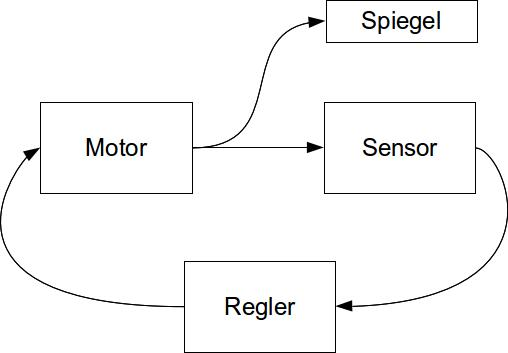
\includegraphics[width=0.6\textwidth]{System_Aufbau.jpg}
	\caption{Allgemeiner Aufbau des simulierten Systems}
	\label{fig:aufbau_system}
\end{figure}

\section{Der Spiegel}
\label{chap:spiegel}
Der Spiegel ist das Bauteil, welches durch den Gleichstrommotor bewegt werden soll.
F�r die Integration in die Simulation m�ssen vorab einige Berechnungen angestellt werden.
Als erstes wird die ben�tigte Beschleunigung berechnet, die mit einem Drehmoment auf den Spiegel �bertragen werden muss, um den Spiegel mit seinem Tr�gheitsmoment �ber 
seinen maximalen Ablenkwinkel zu bewegen.

Dabei werden folgende Vorgaben zu Grunde gelegt:
\begin{itemize}
\item Maximale Ablenkung von $\phi$ = \unit[20}{�} \approx \unit[0,349]{rad}
\item Maximale Zeit f�r Ablenkung \unit[1]{ms}
\item Lineares Modell
\end{itemize}
Berechnung der Winkelgeschwindigkeit:
\begin{center}
\begin{equation}
\label{equ:lineares_motor_model}
\Delta \phi = \unit[20]{�} = \unit[0,349]{rad}\\
\Delta t = \unit[1]{ms} = \unit[0,001]{s}\\
\omega = \frac {\Delta \phi}{\Delta t} = \frac {\unit[0,349]{rad}}{\unit[0,001]{s}} = \unit[349]{rad/s}\\
\end{equation}
\end{center}

Es ergibt sich eine Druchschnittswinkelgeschwindigkeit von \unit[349]{rad/s}, um einen Winkel von \unit[20}{�} in \unit[1]{ms} zu �berfahren.
Dies w�rde aber eine Anfangs- und Endgeschwindigkeit voraussetzen. Da der Spiegel aber aus einer Ruhelage beschleunigt und wieder in einer Ruhelage enden soll, 
wird ein linearer Verlauf der Geschwindigkeit von $\omega = \unit{0}{rad/s}$ und der doppelten Durchschnittsgeschwindigkeit $\omega = \unit{698}{rad/s}$ bei der H�lfte der 
Strecke und bei der Endposition wieder $\omega = \unit{0}{rad/s}$ der zu fahrenden Strecke angenommen. 
Daraus folgt eine Beschleunigung von:
\begin{center}
\begin{equation}
\label{equ:max_alpha_motor}
\Delta \omega = \unit[698]{rad/s}\\
\Delta t = \unit[0,5]{ms} = \unit[0,0005]{s}\\
\\
\alpha = \frac {\Delta \omega}{\Delta t} = \frac {\unit{698}{rad/s}}{\unit{0,0005}{s}} = \unit{1,396 *10^6}{rad/s^2}\\
\end{equation}
\end{center}
Der Spiegel erf�hrt zu Beginn der Regelung eine Beschleunigung von $\alpha = \unit{1,396 *10^6}{rad/s^2}$ um nach der H�lfte der Zeit, also nach \unit[0,5]{ms} wieder mit 
dem gleichen Betrag der Beschleunigung abgebremst zu werden.

Modell f�r den Spiegel:
\begin{itemize}
\item Durchmesser: \unit[12]{mm} --> Radius: R = \unit[6]{mm}
\item H�he: h = \unit[2]{mm}
\item Gewicht: m = \unit[10]{g}
\end{itemize}

Das Tr�gheitsmoment des Spiegels betr�gt demnach: 
\begin{center}
\begin{equation}
\label{equ:J_spiegel}
J = \frac {1} {4} * m * R^2 + \frac{1}{12} * m * h^2\\
J = \frac {1} {4} * \unit[10e-3]{kg} * (\unit[[6e-3]{m})^2 + \frac{1}{12} * \unit[10e-3]{kg} * (\unit[[2e-3]{m})^2\\
J = \unit[93,3e-9]{kgm^2}
\end{equation}
\end{center}

Aus den oben berechneten Daten ergibt sich ein Lastmoment von:
\begin{center}
\begin{equation}
\label{equ:M_last}
M_L = J * \alpha\\
M_L = \unit[93,3e-9]{kgm^2} * \unit[1,396e6]{rad/s^2} \\
M_L = \unit[130,25e-3]{Nm}
\end{equation}
\end{center}

Theoretische Maximale Leistung eines Gleichstrommotors:
\begin{center}
\begin{equation}
\label{equ:max_leistung_motor}
P = M_L * \omega\\
P = \unit[130,25 * 10^{-3}]{Nm} * \unit[698]{rad/s} \\
P = \unit[91]{W}
\end{equation}
\end{center}

\section{Der Motor}
\label{chap:motor}
In der Regel werden Laserablenkespiegel �ber einen Galvo gesteuert. Bei der Bearbeitung dieser Simulationsstudie ergaben sich Probleme, Informationen �ber die Ansteuerung
solcher Galvos zu bekommen. Insofern wird die Simulationsstudie auf der Ansteuerung eines Gleichstrommotors beruhen. Aber auch hierbei konnten jedoch keine Informationen 
�ber die Gleichstrommotorparameter $K_M\phi$ und der Reibungskonstanten bei verschiedenen Herstellern gefunden werden. Um dennoch die Studie durchf�hren zu k�nnen, wird auf die
Motorvorgaben aus der Vorlesung Systemtechnik von Prof. Froriep zur�ck gegriffen.

\subsection{Der elektrische Teil}
\label{chap:elekteil}
Der elektrische Teil eines Gleichstrommotors besteht aus einer Spule $L_A$, ihrem Innenwiderstand $R_A$, der induzierten Spannung $e_A$ und der Eingangsspannung
f�r den Motor $U_e$, siehe Abb. \ref{fig:elekeinzelteil}.
\begin{figure}[!h]
	\centering
	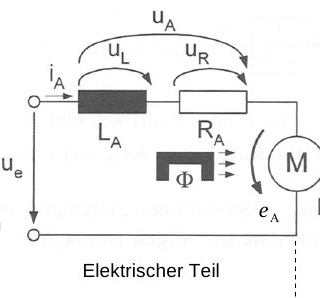
\includegraphics[width=0.6\textwidth]{ElektrischerTeil.jpg}
	\caption{Elektrischer Teil des Motors}
	\label{fig:elekeinzelteil}
\end{figure}
Es l�sst sich folgende Spannungsmasche aufstellen:
\begin{center}
\begin{equation}
\label{equ:motorspannung}
U_e = u_L + u_R - e_A
\end{equation}
\end{center}
Die Spannung $e_A$ wirkt der Eingangsspannung entgegen und hat ein negatives Vorzeichen.
Die Teilspannungen $u_L$ und $u_R$ lassen sich folgenderma�en umschreiben:
\begin{center}
\begin{equation}
\label{equ:motorersatzspannung}
u_L = L_A * si_A \\
u_R = R_A * i_A
s = \frac{d}{dt}
\end{equation}
\end{center}
Dieses l�sst sich in einer Formel ausdr�cken:
\begin{center}
\begin{equation}
\label{equ:motorspannungausfuehrlich}
U_e = L_A * si_A + R_A * i_A - e_A
\end{equation}
\end{center}
F�r die sp�tere Integration in Simulink wird die Gleichung \ref{equ:motorspannungausfuehrlich} umgeschrieben:
\begin{center}
\begin{equation}
\label{equ:motorspannungsimulink}
si_A = \frac{1}{L_A} (e_A - R_Ai_A + u_e)
\end{equation}
\end{center}
Wobei
\begin{center}
\begin{equation}
\label{equ:motorspannungsimulinkkonst}
e_a = K_M * \Phi \omega
\end{equation}
\end{center}
$K_M$ und $\Phi$ Motorkonstanten sind.

\subsection{Der mechanische Teil}
\label{chap:mechteil}
Der mechanische Teil eines Gleichstrommotors besteht aus dem gesamten Drehmoment $M_B$, dem Motormoment $M_M$, dem Lastmoment $M_L$ des Spiegels und der 
Moment-Winkel-Beziehung (Reibung) $M_R = r*\omega$, wobei $\omega = \.\phi$ ist, siehe Abb. \ref{mecheinzelteil}.
\begin{figure}[!h]
	\centering
	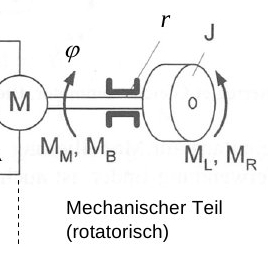
\includegraphics[width=0.6\textwidth]{MechanischerTeil.jpg}
	\caption{Mechanischer Teil des Motors}
	\label{fig:mecheinzelteil}
\end{figure}
Es l�sst sich folgende Moment-Bilanzgleichung aufstellen:
\begin{center}
\begin{equation}
\label{equ:motormomentebilanz}
M_B = M_M - M_R - M_L = \\
J * s\omega = M_M - r * \omega - M_L\\
s = \frac{d}{dt}
\end{equation}
\end{center}
F�r die sp�tere Integration in Simulink wird die Gleichung \ref{equ:motormomentebilanz} umgeschrieben:
\begin{center}
\begin{equation}
\label{equ:motormomentsimulink}
s\omega = \frac{1}{J} (M_M - r * \omega - M_L)
\end{equation}
\end{center}
Wobei
\begin{center}
\begin{equation}
\label{equ:motormomentsimulinkkonst}
M_M = K_M * \Phi *i_A
\end{equation}
\end{center}
$K_M$ und $\Phi$ Motorkonstanten sind.

\subsection{Der ganze Motor}
\label{chap:ganzermotor}
Werden die beiden Einzelaspekte des Motors gleichzeitig betrachtet, so ergbit sich folgender Zusammenhang wie er in Abb. \ref{fig:motoraufbau} dargestellt ist.
\begin{figure}[!h]
	\centering
	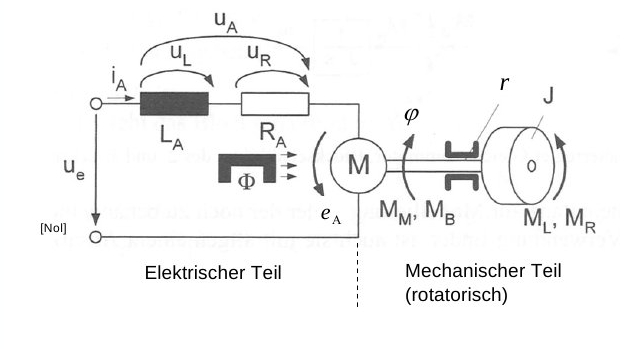
\includegraphics[width=0.6\textwidth]{Motoraufbau.jpg}
	\caption{Aufbau des Motors}
	\label{fig:motoraufbau}
\end{figure}

\section{Der Sensor}
\label{chap:sensor}
Im Folgenden werden der Aufbau, das physikalische Modell, sowie verschiedene mathematische Modelle des Sensors vorgestellt und erl�utert.

\subsection{Das physikalische Modell des Sensors}
\label{chap:physik_modell_sensor}
Der in Abb. \ref{fig:aufbau_system} dargestellte Sensor, gliedert sich nach folgender Darstellung in Abb. \ref{fig:aufbau_sensor} auf in:
\begin{itemize}
	\item{Einer Lichtquelle: LED}
	\item{Einer Blende mit einer Transmissionsfunktion $T(\varphi)$}
	\item{Einer Anordnung aus Photodioden, welche die transmittierte Lichtleistung als Spannungssignal $U_{ph} (\phi)$ bzw. $U_{ph} (\varphi)$ darstellt}
\end{itemize}

\begin{figure}[ht]
	\centering
	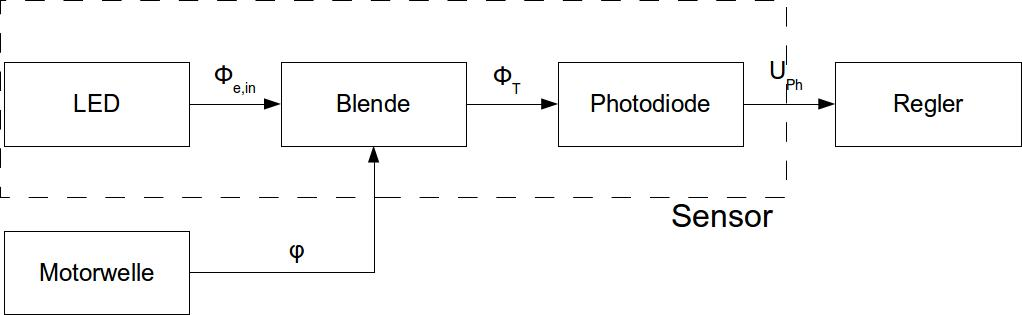
\includegraphics[width=0.8\textwidth]{Sensor_Aufbau.jpg}
	\caption{Allgemeiner Aufbau des Sensors}
	\label{fig:aufbau_sensor}
\end{figure}

\underline{\textbf{Die LED}}\\
Die LED wird im folgenden als ein punktf�rmiger, Lambert'scher Strahler betrachtet. Die gesamte Strahlungsleistung $\phi_e$ wird in den Halbraum $\omega = 2\pi$ abgestrahlt. 
Somit ergibt sich nach \citep{}%quelle f�r Abstrahlcharakteristik einf�gen
folgendem Zusammenhang:
\begin{equation}
\label{equ:abstrahl_charakteristik}
BLABLUB
\end{equation}




\subsection{Das lineare Sensormodell}
\label{chap:linear_sensor}


\subsection{Das nicht lineare Sensormodell}
\label{chap:nonlinear_sensor}
\newpage
%\null
%\cleardoublepage



%************************************************************************************************
% Kap.4 Programmentwicklung
%************************************************************************************************

\chapter{Programmentwicklung}
\label{chap:Programmentwicklung}
Bei der Programmentwicklung werden die in Kap. \ref{chap:modellbildung} aufgestellten Gleichungen mit Matlab und Simulink umgesetzt.
Es wird begonnen, die Gleichungen des elektrischen und des mechanischen Teils des Motors in Simulink umzusetzen.
Im Anschluss folgt die Implementierung der Werte, des Simulinkprogrammes und des Motors in Matlab.
Daran schliesst sich die Umsetzung der Sensoren in Matlab.
Wenn die Sensoren mit Matlabfiles eingebunden werden k�nnen, werden die Simulink- und Matlabprogramme des Motors entsprechend erweitert.

\section{Motor in Simulink}
\label{chap:motorinsimulink}
Es werden die Formeln \ref{equ:motorspannungsimulink} und \ref{equ:motormomentsimulink} aus den Kap. \ref{chap:elekteil} und \ref{chap:mechteil} hergenommen.
Durch ein umstellen der beiden Formeln, so dass nur noch erste Ableitungen in beiden Formeln vorkommen, lasen sie sich kombinieren und in Simulink einbinden, da so ein
Gleichungssytem nur mit ersten Ableitungen entstanden ist.
Um einen besseren �berblick zu bekommen, werden die Formeln hier noch einmal aufgef�hrt.
\begin{center}
\begin{equation}
\label{equ:motorspannungsimulink2}
si_A = \frac{1}{L_A} (e_A - R_Ai_A + u_e)
\end{equation}
\end{center}
\begin{center}
\begin{equation}
\label{equ:motorspannungsimulinkkonst2}
e_a = K_M * \Phi \omega
\end{equation}
\end{center}
\begin{center}
\begin{equation}
\label{equ:motormomentsimulink2}
s\omega = \frac{1}{J} (M_M - r * \omega - M_L)
\end{equation}
\end{center}
\begin{center}
\begin{equation}
\label{equ:motormomentsimulinkkonst2}
M_M = K_M * \Phi *i_A
\end{equation}
\end{center}
$K_M$ und $\Phi$ sind Motorkonstanten.

Mit der Annahme das 
\begin{center}
\begin{equation}
\label{equ:variablensimulink1}
x_1 := \omega
\end{equation}
\begin{equation}
\label{equ:variablensimulink2}
x_2 := i_A
\end{equation}
\end{center}
ist, l�sst sich folgendes Gleichungssytem aufstellen:
\begin{center}
\begin{equation}
\label{equ:motormomentsimulink1}
\dot{x_1} = \frac{1}{J} (K_M \Phi x_Sensor_Funktion2 - r * x_1 - M_L)
\end{equation}
\begin{equation}
\label{equ:motormomentsimulink1}
\dot{x_2} = \frac{1}{L_A} (K_M * \Phi x_1 - R_Ax_2 + u_e)
\end{equation}
\end{center}
Dieses Gleichungssytem l�sst sich jetzt durch die grafischen Elemente in Simulink sehr einfach modellieren.

Wie zu Begin des Kap. \ref{chap:motor} erw�hnt, war es nicht m�glich an verschiedene Werte der Motorkonstanten $K_M$ und $\phi$ zu gelangen.
Aus diesem Grund wird auf die begleitenden Unterlagen der Vorlesung Systemtechniken von Prof. Froriep zur�ck gegriffen.

Auf dieser Grundlage werden die weiteren Programme entwickelt.

Um eine Regelung aufzubauen, wird noch ein Regler, ein Sollwertgeber und ein Subtrahierer von Ist- und Sollwert ben�tigt.
Diese werden �ber die Simulinkbibliothek eingebunden und entsprechende Verbindungen werden angelegt.
Das fertige Grundprogramm ist in Abb. \ref{fig:grundprogramm} dargestellt.
\begin{figure}[!h]
	\centering
	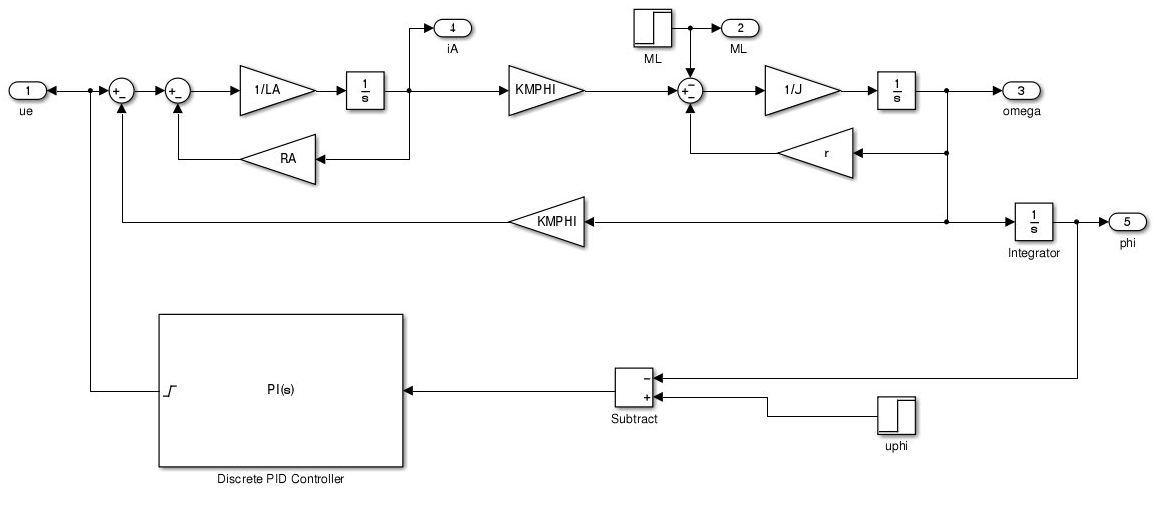
\includegraphics[width=0.6\textwidth]{sSpiegel.jpg}
	\caption{Simulink Grundprogramm}
	\label{fig:grundprogramm}
\end{figure}

\section{Matlab}
\label{chap:Matlab}
\subsection{Motor in Matlab}
\label{chap:motor_matlab}
Die Programmentwicklung in Matlab gestaltet sich f�r den Motor als relativ einfach, da, wie oben erw�hnt, keien Motordaten gefunden wurden, wird auf das Matlabfile von Prof. Froriep aus der Vorlesung "Systemtechniken" zur�ck gegriffen.
In diesem Matlabfile stehen:
\begin{itemize}
\item Die Motorkenndaten
\item Die berechnete Tr�gheit des Spiegels
\item Das berechnete Drehmoment
\item Die Grenzen f�r die Plots
\item Die Anweisungen f�r die Plots
\item Die Anweisungen f�r den Integrationsalgorithmus.
\end{itemize}

Dieses File ist eine sehr gute Grundlage f�r die Simuation, welches w�hrend der Simulation entsprechend angepasst werden kann.

Als Gr��en zur Ausgabe in einem Diagramm, interessieren vor allem die Eingangsspannung $u_e$, der aktuelle Winkel $\phi$, sowie der Sollwinkel mit seinen Toleranzen.
Es werden drei Plots dargestellt.
In dem ersten Plot ist die Motorspannung dargestellt.
In dem zweiten Plot der aktuelle Winkel $\phi$, der direkt von dem Motor abgegriffen wird, sowie der einzustellende Sollwinkel dargestellt.
Der dritte Plot enth�lt auch wieder den aktuellen Winkel $\phi$, jedoch mit einer feineren Aufl�sung um den Sollwinkel, um die Toleranzgrenzen besser erkennen zu k�nnen.

\subsection{Sensor in Matlab}
\label{chap:sensor_matlab}
Der Sensor selbst wird nur mit Matlabprogrammen simuliert.
Dies erm�glicht verschiedene Sensoren in das Hauptprogramm einzubinden und �nderungen an z.B. den Ausma�en und dem Verhalten des Sensors vorzunehmen, ohne das Hauptprogramm �ndern zu m�ssen.

\subsubsection{Sensorkonstanten}
\label{chap:sensorkonstanten}
Um einen Sensor mit seinen verschiedenen Kenngr��en wie Sensorfl�che, �bertragungsverhalten, und weiteres simulieren zu k�nnen, werden die verschiedenen Funktionen aus Kap. \ref{chap:sensor} in einzelnen Matlabfiles umgesetzt. Die Charakteristischen Daten der Photodioden, Blende und LED werden mit Hilfe der Matlabfunktion \texttt{SensorDaten.m} (siehe Anhang \ref{app:sensorDatenM}) in ein Cell-Array gespeichert. Dies Bietet den Vorteil, die Ergebnisse komplizierter Berechnungen und einige Konstanten in einer einzigen Variable zu speichern und an die Hauptfunktion \texttt{sensor.m} zu �bergeben.

Die in Kap. \ref{chap:nonlinear_sensor} erl�uterte mathematische Beschreibung der Einfl�sse von Beugung und Streulicht, wird in den Zeilen 38 bis 81 der Matlab-Funktion umgesetzt.
Die limitierung auf eine Diskrete Faltungsoperation erzeugt bei der Umsetzung einige Probleme.
\begin{itemize}
\item Diskrete Faltung erzeugt Randeffekte (Abweichung zur kontinuierlichen L�sung der Faltung zweier Rechteckfunktionen) -> Definitionsbereich vergr��ern
\item Diskrete Faltung erzeugt Diskrete L�sung. Somit muss das Verhalten des Sensors zwischen den L�sungswerten der Faltung interpoliert werden -> lineare Interpolation
\end{itemize}

\subsubsection{Rechtecks- und Gl�ttungsfunktion}
\label{chap:recht_glatt}
Die Berechnung der Diskreten Faltung ben�tigt Diskrete Funktionswerte der Rechteckfunktionen f�r Blende und Dioden. Die im Anhang \ref{app:frectM} und \ref{app:gekernM} dargestellten Matlab-Files \texttt{frect.m} und \texttt{gekern.m} Berechnen die Funktionswerte der in Kap. \ref{chap:nonlinear_sensor} beschriebenen Funktionen. Diese werden im File \texttt{SensorDaten.m} (vgl. Kap. \ref{chap:sensorkonstanten}) in For-Schleifen zu Vektoren mit Diskreten Funktionswerten zusammengesetzt.

\subsubsection{Die Sensor-Funktion}
\label{chap:sensorM}
Die Verwendungs des Sensors in den vorhandenen Simulinkprogramme macht es n�tig, diverse Voreinstellungen als globale Variablen zu �bergeben.
\begin{itemize}
\item \texttt{Unit}: die Einheit, in der die Sensorfunktion den Positionswinkel der Motorwelle �bergeben wird
\item \texttt{mode}: das �bertragungsverhalten, des Sensors
\item \texttt{Sensorkonstanten}: die in Kap. \ref{chap:sensorkonstanten} beschriebenen charakteristischen Werte des Sensorsystems als Cell-Array
\end{itemize}

Die Variable \texttt{Unit} erm�glicht eine Umrechnung der Einheit f�r den eingegebenen Motorwellenwinkel.

Um das Wirken, des Differenzenprinzips in der Vorliegenden Anordnung zu demonstrieren, wird ein Rauschen generiert. Dieses variiert statistisch gleichverteilt im bereich von 0 bis $\frac{1}{10}$ des maximalen Stromsignals.

Die in Kap. \ref{chap:sensor} vorgestellten Mathematischen Modelle werden mittels caseswitch der Variablen \texttt{mode} implementiert. F�r die modes: \glqq linear2 \grrq und \glqq nonlinear \grrq m�ssen die Funktiondswerte, welche zwischen den diskreten, charakteristischen werten liegen linear interpoliert werden.

\subsubsection{Die Plausibilit�tstests zum Sensor}
\label{chap:sensor_plausile}
Hier soll das in Kap. \ref{chap:nonlinear_sensor} beschriebene verhalten, bei Beeinflussung der Messung durch Streulicht und Beugung qualitativ bewertet und auf Plausibilit�t gepr�ft werden.
Abb. \ref{fig:diode_faltung} Zeigt den Verlauf der Gewichtungsfunktion(Faltungsfunktion) �ber den Azimutwinkel bzw. Positionswinkel $\varphi$

\begin{figure}[!h]
	\centering
	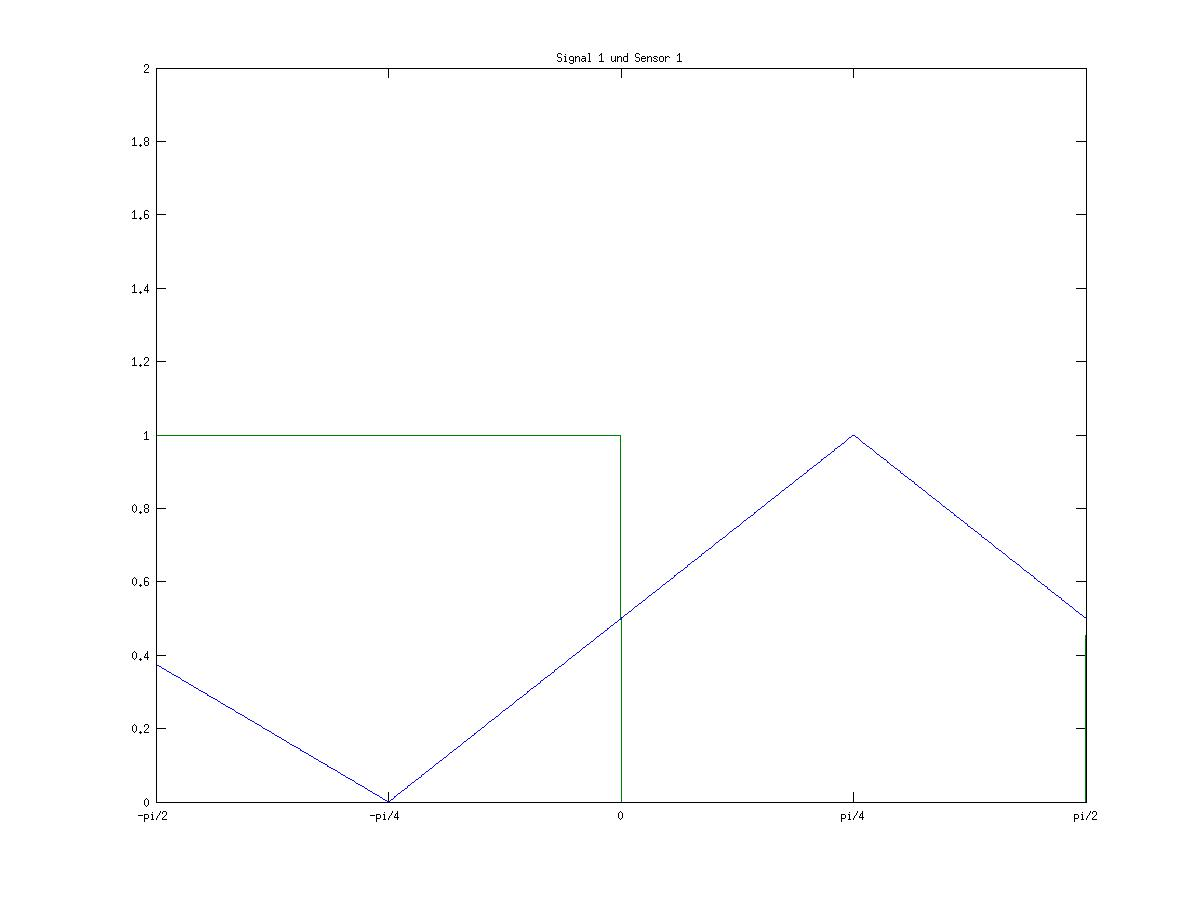
\includegraphics[width=0.6\textwidth]{../Plots/figure_4.jpg}
	\caption{Diodenfunktion und lineare Faltungsfunktion}
	\label{fig:diode_faltung}
\end{figure}
\FloatBarrier

Abb. \ref{fig:vergleich_lin_glatt} zeigt, dass die diskrete Faltung der Blenden- und der Diodenfunktion qualitativ das erwartete Verhalten abbildet.
\begin{figure}[!h]
	\centering
	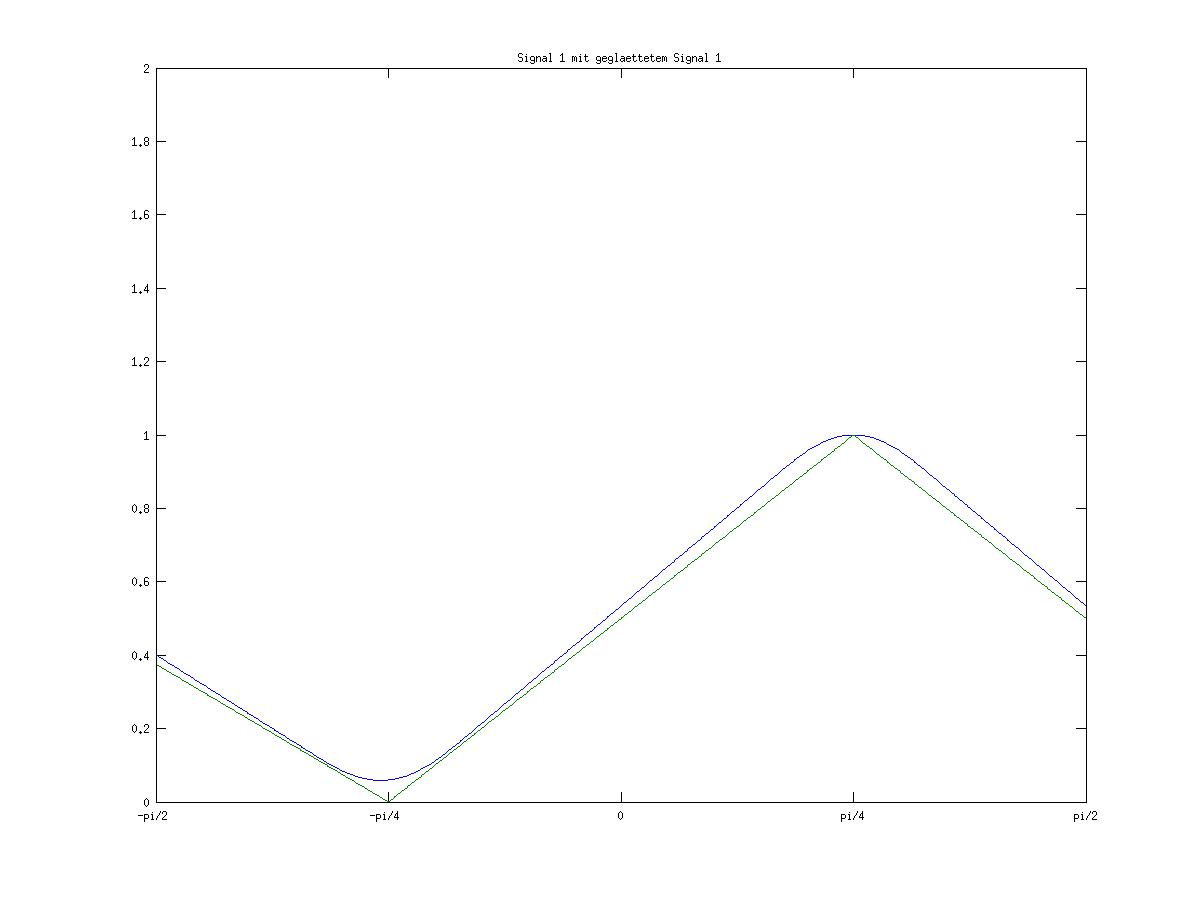
\includegraphics[width=0.6\textwidth]{../Plots/figure_8.jpg}
	\caption{Vergleich der ungegl�tteten mit der gegl�tteten Funktion}
	\label{fig:vergleich_lin_glatt}
\end{figure}
\FloatBarrier

Im folgenden soll �berpr�ft werden, ob die Sensoren f�r den maximalen Messbereich von $\pm \unit[45]{�}$ das erwartete Verhalten Zeigen.
Abb. \ref{fig:kennlinie_einzelgruppe} zeigt die Kennlinie einer einzelnen Diodengruppe mit Einfluss durch statistisch gleichverteiltes Rauschen.
\begin{figure}[!h]
	\centering
	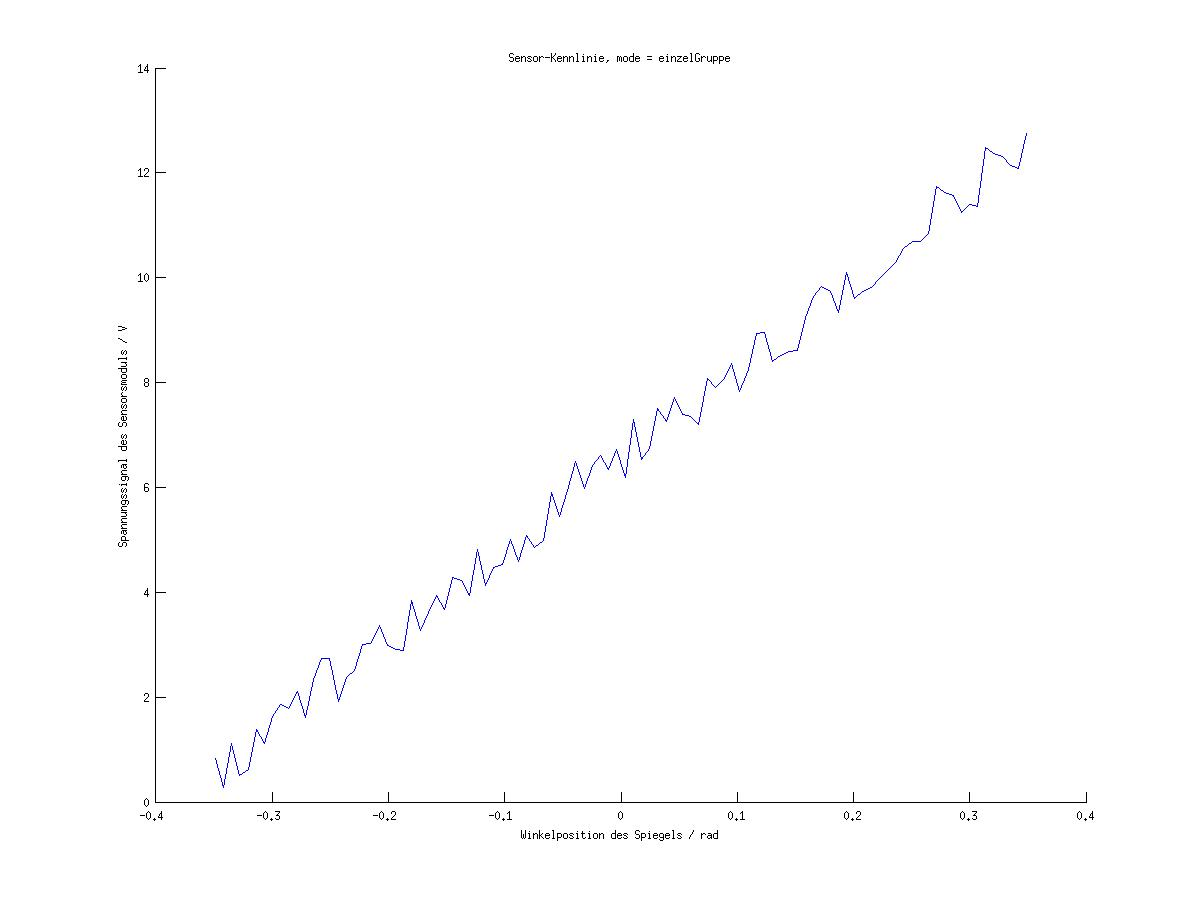
\includegraphics[width=0.6\textwidth]{../Plots/Sensor-Kennlinie_einzelGruppe.jpg}
	\caption{Kennlinie des Sensors im mode: einzelGruppe}
	\label{fig:kennlinie_einzelgruppe}
\end{figure}
\FloatBarrier

Abb. \ref{fig:kennlinie_linear1} zeigt, das ideal lineare Verhalten des Sensors im mode: linear1.
\begin{figure}[!h]
	\centering
	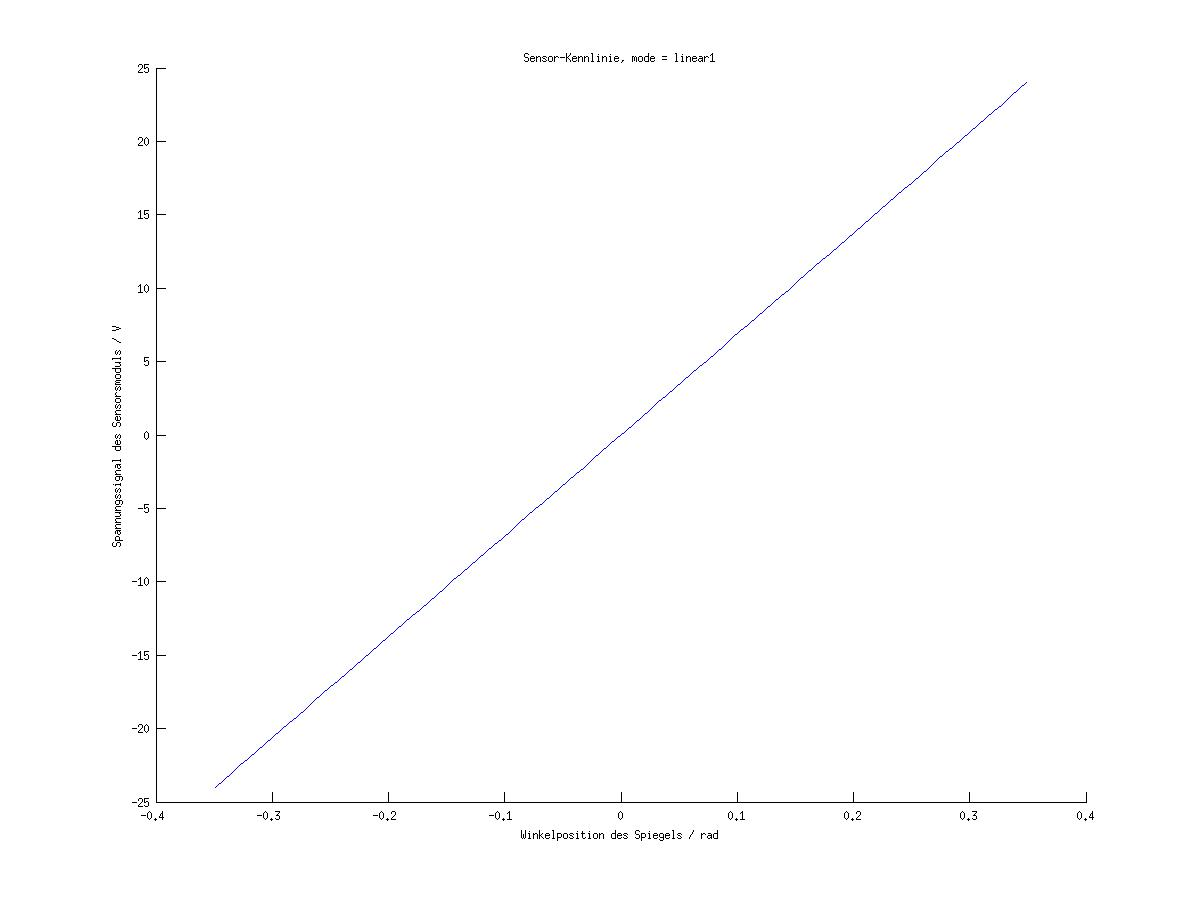
\includegraphics[width=0.6\textwidth]{../Plots/Sensor-Kennlinie_linear1.jpg}
	\caption{Kennlinie des Sensors im mode: linear1}
	\label{fig:kennlinie_linear1}
\end{figure}
\FloatBarrier

Abb. \ref{fig:kennlinie_linear2} stellt die Kennlinie des Sensors mittels Faltungsfunktion ohne Gl�ttung wie erwartet dar.
\begin{figure}[!h]
	\centering
	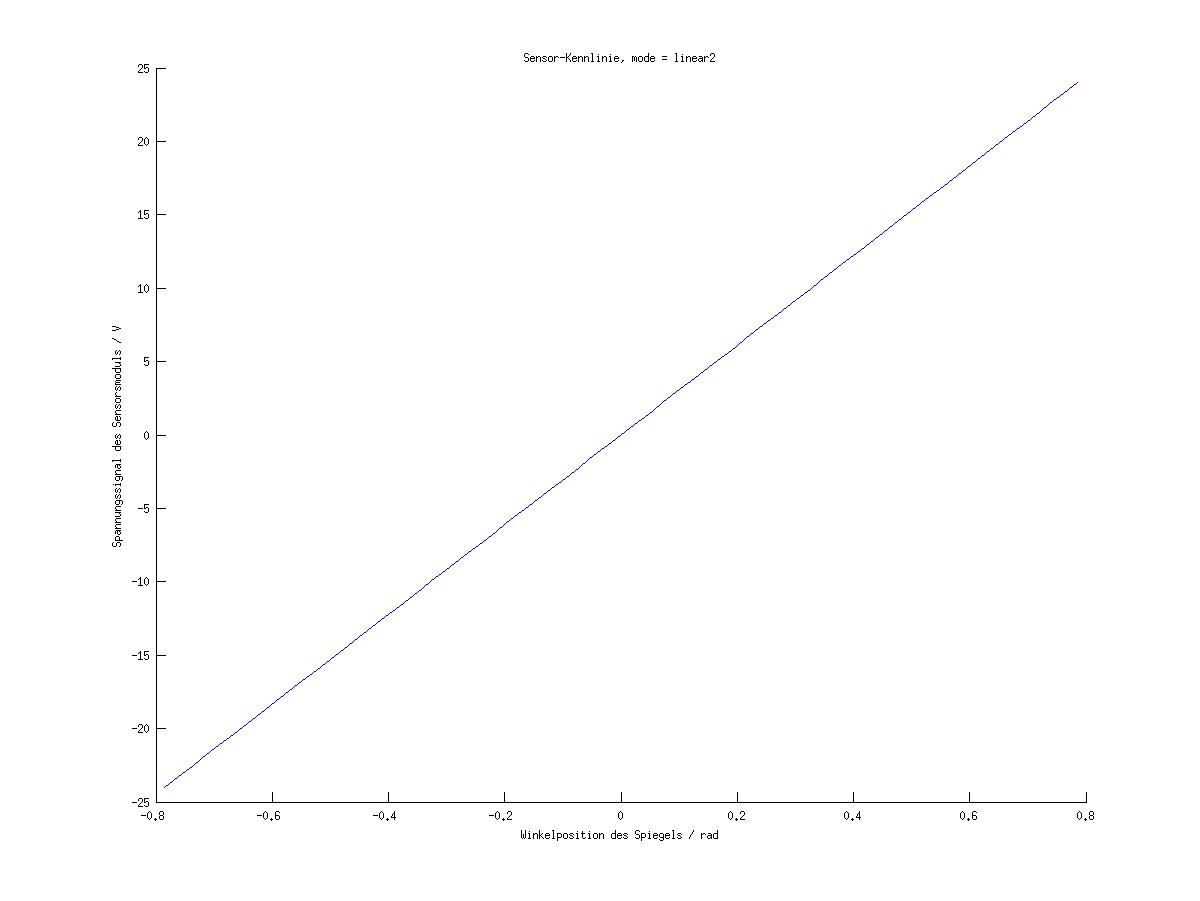
\includegraphics[width=0.6\textwidth]{../Plots/Sensor-Kennlinie_linear2.jpg}
	\caption{Kennlinie des Sensors im mode: linear2}
	\label{fig:kennlinie_linear2}
\end{figure}
\FloatBarrier

Eben falls im mode: nonlinear zeigt die Abb. \ref{fig:kennlinie_nonlinear} qualitativ das erwartete Verhalten der Kennlinie.
\begin{figure}[!h]
	\centering
	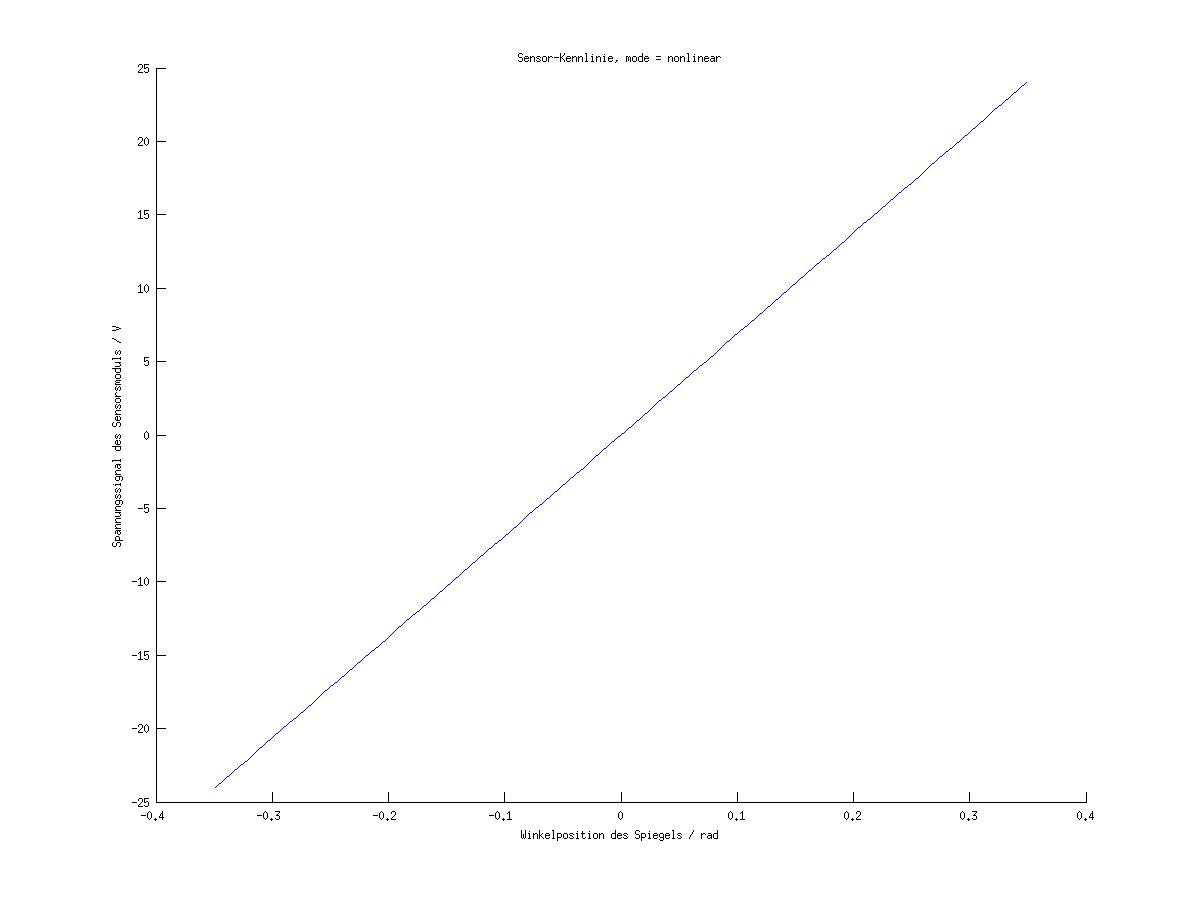
\includegraphics[width=0.6\textwidth]{../Plots/Sensor-Kennlinie_nonlinear.jpg}
	\caption{Kennlinie des Sensors im mode: nonlinear}
	\label{fig:kennlinie_nonlinear}
\end{figure}
\FloatBarrier
\newpage
%\null
%\cleardoublepage



%************************************************************************************************
% Kap65 Simulationsdurchf�rhung
%************************************************************************************************

\chapter{Simulationsdurchf�hrung}
\label{chap:Simulationsdurchfuehrung}

In diesem Abschnitt werden verschiedene Simulationen durchgef�hrt.
Der Motor, der der Regelung zu Grunde liegt, ist der Gleichstrommotor aus der Vorlesung von Prof. Froriep.
Mit diesem Motor soll von einer Nullposition ausgehend ein Winkel von 20{\textdegree} angefahren werden. Dieser Winkel soll innerhalb von einer Millisekunde erreicht werden.

Es wird eine Spannungsbegrenzung von +/- 24 V eingef�hrt, da diese eine in der Fertigung �bliche Versorgungsspannung ist.

Zu Beginn wird der Sensor, der das aktuelle Positionssignal liefert, aus der Regelung heraus gelassen. Somit ist es m�glich, die Regelung an den Motor anzupassen und sobald
diese die Sollwerte erf�llt, werden 2 verschiedene Sensoren das Positionssignal liefern.

F�r die verschiedenen P-, PI-, PD- und PID-Regelungen wird der PID-Reglerblock von Simulink verwendet.

Es wird mit einer P-Regelung begonnen, die Sollwerte zu erreichen. Wenn die P-Regelung nicht ausreicht, wird die P-Regelung erst nur um einen I-Anteil und dann nur um einen 
D-Anteil erweiteret. Sollten immernoch keine Zufriedenstellenden Ergebnisse vorliegen, so wird mit einer PID-Regelung versucht, die Vorgaben zu erreichen.

In Abb. \ref{p40} ist das Ergebnis der reinen P-Regelung dargestellt. Es ist zu erkennen, dass nach ca. 7 ms es keine Ver�nderung des eingesetllten Winkels gibt. Eine 
Erh�hung des P-Anteils ergibt ein �berschwingen, wie es in Abb. \ref{p45} dargestellt ist.
In Abb. \ref{p40} und \ref{p45} ist in der untersten Grafik der Sollwinkel sowie die angegebene Abweichung angezeigt. Wie zu erkennen ist, ist die verbleibende Regeldifferenz noch viel 
zu gro�. Demnach wird mit einem zugef�gten I-Anteil zur reinen P-Regelung versucht, die restliche gro�e Regeldifferenz auszugleichen. 
F�r die folgenden Simulationen wird das Matlab-File "msSpiegel_PID.m" und das Simulink-File "sSpiegel.slx" hergenommen.

\begin{figure}[!h]
	\centering
	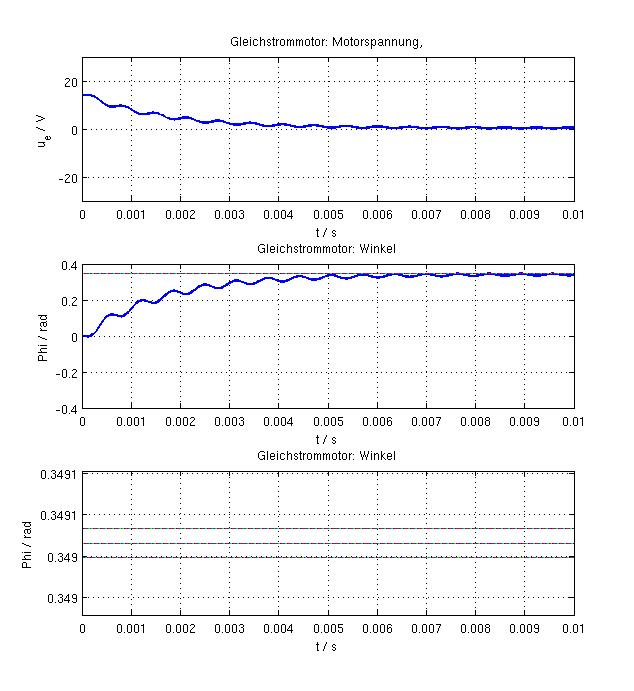
\includegraphics[width=0.6\textwidth]{NurP40.jpg}
	\caption{P-Anteil von 40}
	\label{p40}
\end{figure}

\begin{figure}[!h]
	\centering
	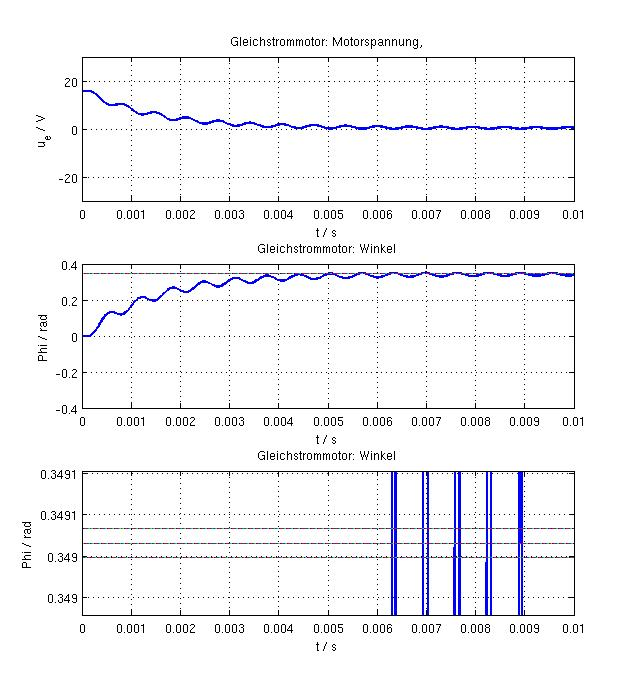
\includegraphics[width=0.6\textwidth]{NurP45.jpg}
	\caption{P-Anteil von 45}
	\label{p45}
\end{figure}

In Abb. \ref{p30i17} ist das Ergebnis der PI-Regelung dargestellt. Es ist zu erkennen, dass nach ca. 13 ms es keine Ver�nderung des eingesetllten Winkels gibt. Eine Erh�hung 
des P- oder I-Anteils ergibt ein �berschwingen, wie es in Abb. \ref{p30i17} dargestellt ist.
In Abb. \ref{p30i17} und \ref{p30i17} ist in der untersten Grafik der Sollwinkel sowie die angegebene Abweichung angezeigt. Wie zu erkennen ist, ist die verbleibende Regeldifferenz noch viel 
zu gro�. 
Demnach wird der zugef�gte I-Anteil herausgenommen und ein D-Anteil zur reinen P-Regelung hinzugenommen, um so ein besseres Regelergebnis zu erreichen.

\begin{figure}[!h]
	\centering
	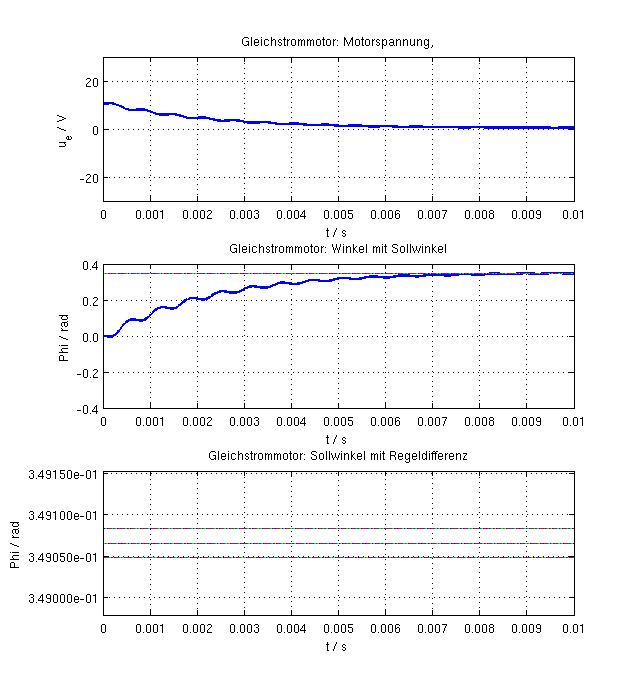
\includegraphics[width=0.6\textwidth]{PI-P30I17.jpg}
	\caption{P-Anteil von 30 und I-Anteil von 17}
	\label{p30i17}
\end{figure}

\begin{figure}[!h]
	\centering
	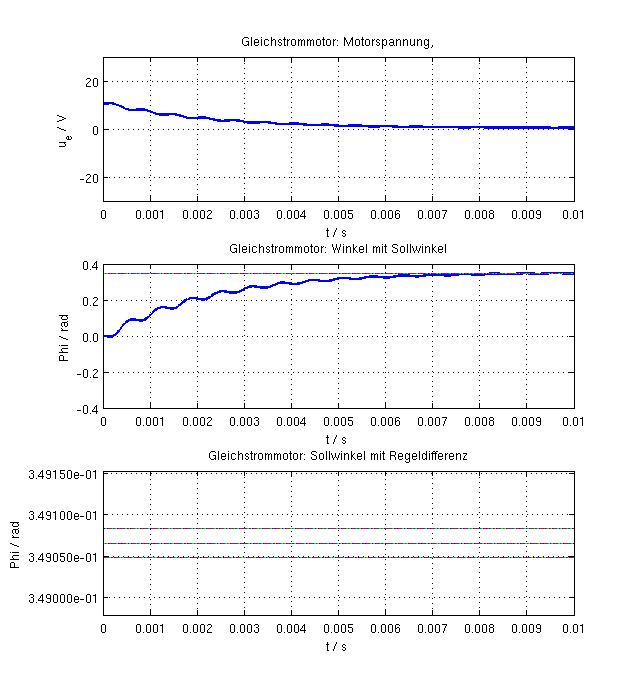
\includegraphics[width=0.6\textwidth]{PI-P30I17.jpg}
	\caption{P-Anteil von 30 und I-Anteil von 17}
	\label{p30i17}
\end{figure}

Auch mit der PD-Regelung werden die Vorgaben noch nicht erf�llt. 
In Abb. \ref{p22d1n1} ist das Ergebnis der PD-Regelung dargestellt. Es ist zu erkennen, dass nach ca. 7 ms es keine Ver�nderung des eingesetllten Winkels gibt. Eine Erh�hung 
des P- oder D-Anteils ergibt ein �berschwingen, wie es in Abb. \ref{p23d1n1} dargestellt ist.
In Abb. \ref{p22d1n1} und \ref{p23d1n1} ist in der untersten Grafik der Sollwinkel sowie die angegebene Abweichung angezeigt. Wie zu erkennen ist, ist die verbleibende Regeldifferenz noch viel 
zu gro�. 

\begin{figure}[!h]
	\centering
	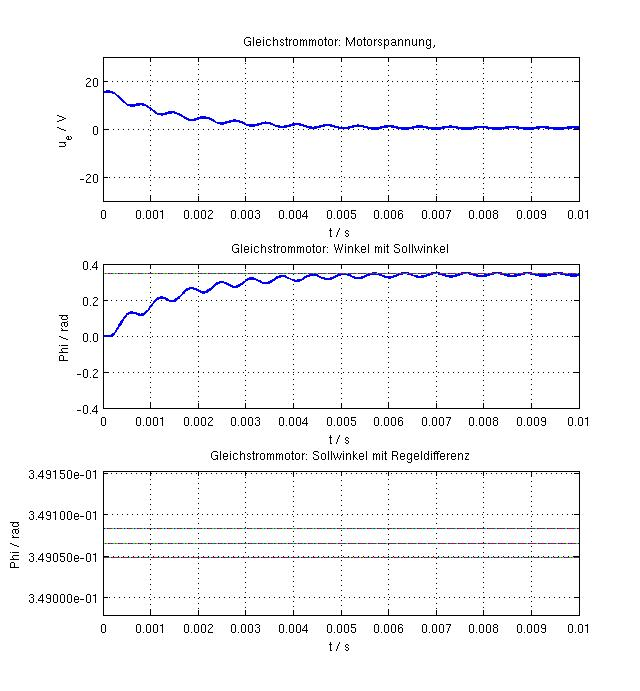
\includegraphics[width=0.6\textwidth]{PD-P22D1N1.jpg}
	\caption{P=22 - D=1 - N=1}
	\label{p22d1n1}
\end{figure}

\begin{figure}[!h]
	\centering
	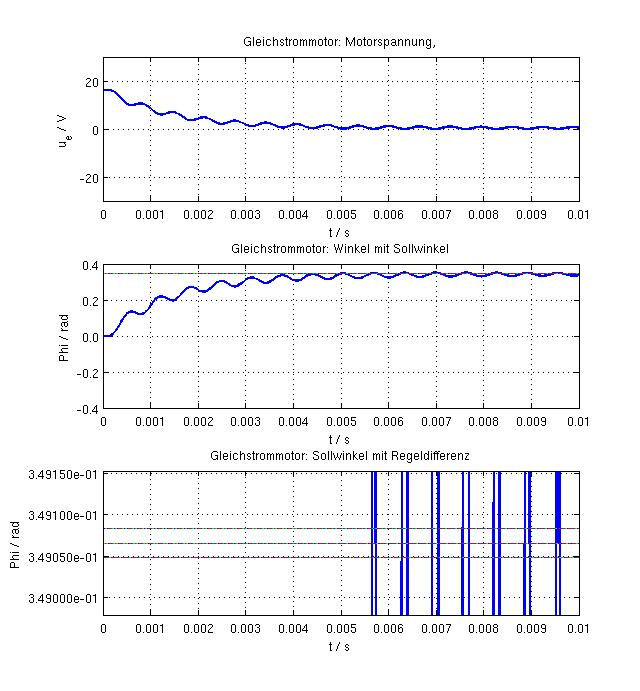
\includegraphics[width=0.6\textwidth]{PD-P23D1N1.jpg}
	\caption{P=22 - D=1 - N=1}
	\label{p23d1n1}
\end{figure}

Nun wird mit einer Kombination der P-, I- und D-Anteile die Regelung betrieben.
In Abb. \ref{p20i16d1n1} ist das Ergebnis der PID-Regelung dargestellt. Es ist zu erkennen, dass nach ca. 7 ms es keine Ver�nderung des eingesetllten Winkels gibt. Eine Erh�hung 
der verschiedenen Reglerparamteranteile ergibt ein �berschwingen, wie es in Abb. \ref{p20i16d1n1} dargestellt ist.
In Abb. \ref{p20i16d1n1} ist in der untersten Grafik der Sollwinkel sowie die angegebene Abweichung angezeigt.
Durch die gro�e Abweichung vom Sollwinkel ist in dieser Grafik kein Graph zu erkennen.

\begin{figure}[!h]
	\centering
	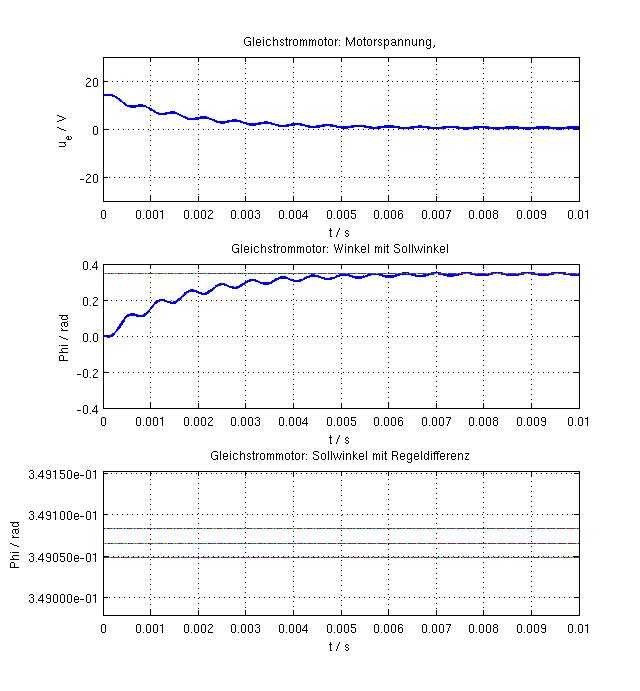
\includegraphics[width=0.6\textwidth]{PID-P20I15D1N1.jpg}
	\caption{P=20 - I=15 - D=1 - N=1}
	\label{p20i15d1n1}
\end{figure}

\begin{figure}[!h]
	\centering
	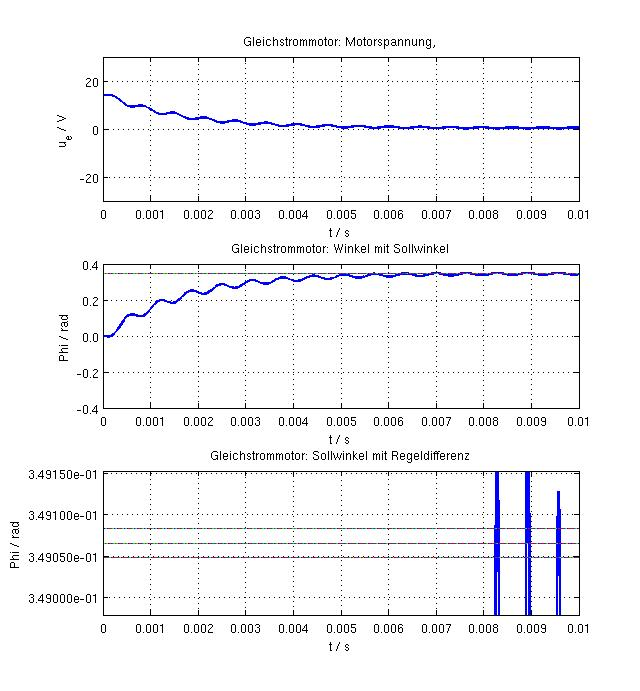
\includegraphics[width=0.6\textwidth]{PID-P20I16D1N1.jpg}
	\caption{P=20 - I=16 - D=1 - N=1}
	\label{p2oi16d1n1}
\end{figure}


Es zeigt sich, dass der P-Anteil den meisten Einfluss, bzw. den gr��ten Erfolg bei der Regelung ausmacht. Durch hinzugef�gte I- oder D-Anteile konnte die Regelung nicht
verbessert werden.
Nach dem die verschiedenen Regler die Vorgaben noch nicht erf�llen konnten, wird nun die P-Adapion eingesetzt. Bei der P-Adaption wird folgende Formel vor den P-Verst�rker 
geschaltet:
 
\begin{center}
\begin{equation}
f = 1 + \frac {c_1 - 1}{(c_2 * e)^2 + 1}
\end{equation}
\end{center}
 
Dabei muss der Regelkreis folgenderma�en erweitert werden:
 
\begin{figure}[!h]
	\centering
	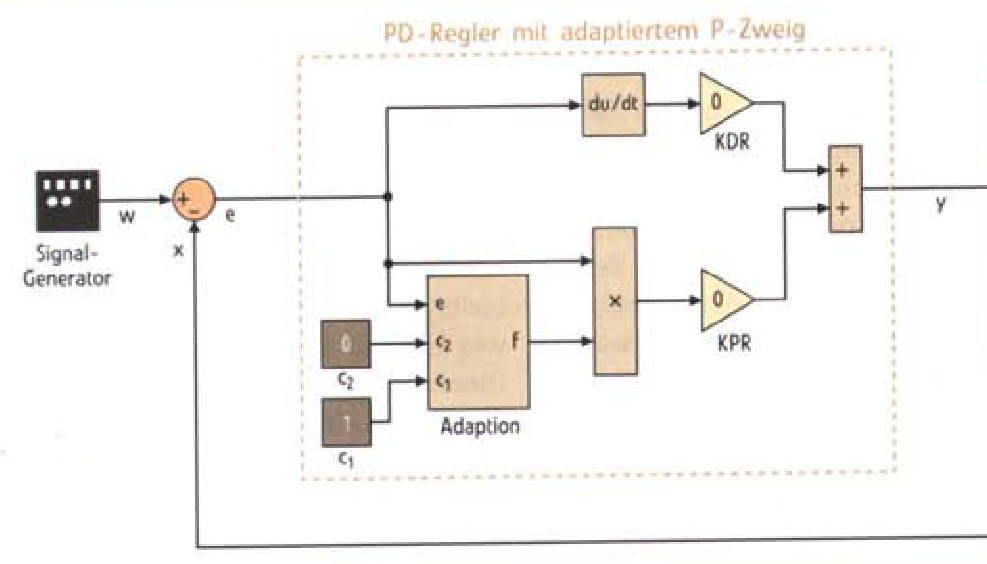
\includegraphics[width=0.6\textwidth]{P-Adaption.jpg}
	\caption{P-Adaption}
	\label{padaption}
\end{figure}

Quelle: PDF, "Tempo beim Laserzugriff", Artikel im F&M Elektronik, Jahrg.111(2003)5, Lugmair, Froriep, Kuplent, Langhans

Nun kann mit drei verschiedenenn Parametern verucht werden, die Sollwerte zu erreichen.
Wobei die beiden f-Parameter zu Beginn auf 1 gesetzt werden und erst mit dem erh�hen des P-Anteils versucht wird, eine gute Regelung zu erhalten. Danch werden die beiden
f-Parameter einzeln erh�ht bzw. erniedrigt, bis sich das Erebniss verbessert hat. Eine Anpassung des P-Anteils und danach eine erneute Anpassung der f-Parameter geh�rt 
ebenso zur Erreichung einer passenden Regelung.
F�r die folgenden Simulationen wird das Matlab-File "msSpiegel_Pad.m" und das Simulink-File "sSpiegelPad.slx" hergenommen.

\begin{figure}[!h]
	\centering
	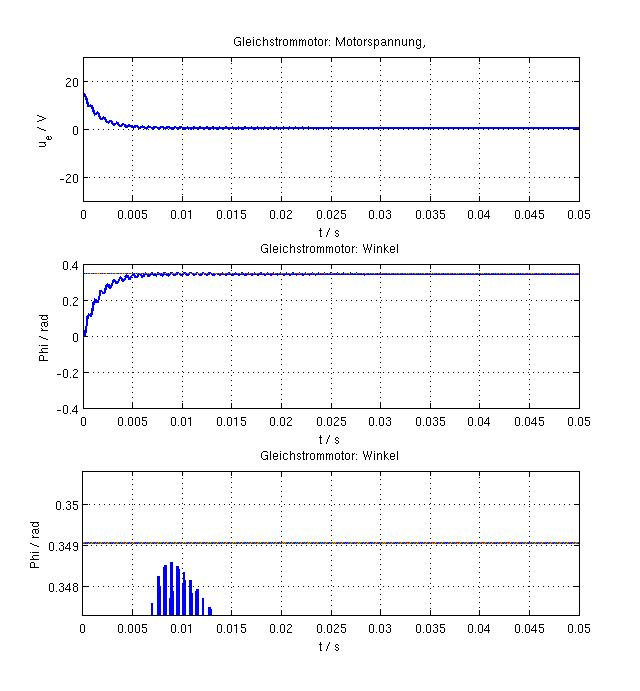
\includegraphics[width=0.6\textwidth]{Pad-P41F1_1,5F2_80.jpg}
	\caption{P-Adaption mit Parametern}
	\label{padp41f1580}
\end{figure}

In Abb. \ref{padp41f1580} ist zu erkennen, dass der Sollwinkel nicht erreicht wird. Wird jedoch der P-Anteil erh�ht und mit den beiden f-Parametern weitere Einstellungen
probier, so wird der Sollwinkel nie erreicht. Es kommt zwar zu einem Schwingen um den Sollwinkel, aber dieser kann nicht stabil erreicht werden, siehe Abb. \ref{padp50f3400}.

\begin{figure}[!h]
	\centering
	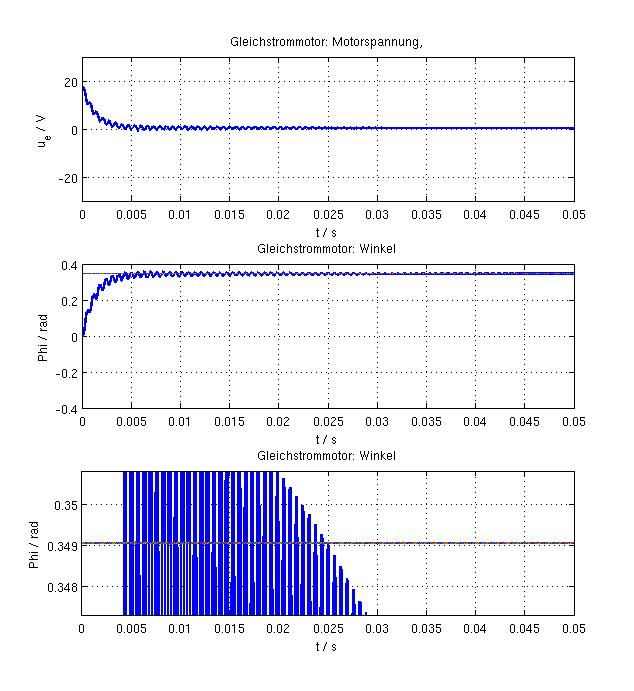
\includegraphics[width=0.6\textwidth]{Pad-P50F1_3F2_400.jpg}
	\caption{P-Adaption mit Parametern}
	\label{padp50f3400}
\end{figure}

Durch die Verwendung der P-Adaption konnte die Einregelzeit nicht verbessert werden.
Es zeigt sich, dass mit dem vorhandenen Gleichstrommoter keine der Vorgaben eingehalten werden k�nnen.
Um heraus zu finden, welche Daten der Motor aufweisen m�sste, um mit einer PID- oder P-Adaption geregelt werden zu k�nnnen, werden jetzt zus�tzlich zu den $f_{1}$ und $f_{2}$
Parametern auch die Motorparameter ge�ndert.
Beispielhaft wurden Werte f�r den Innenwiderstand und der Induktivit�t eines Galvos 6230 der Firma Cambridge Technology als Grundlage verwendet.

Quelle: PDF, Model 6230H Optical Scanner (Mechanical and Electrical Specifications), Cambridge Technology, 03/07.

F�r die folgenden Simulationen wird das Matlab-File "msSpiegel_Pad_Werte.m" und das Simulink-File "sSpiegelPad.slx" hergenommen.

In Abb. \ref{padwerte} ist eine langsame Ann�herung an die zu erf�llenden Vorgaben zu sehen. Jedoch noch nicht in der geforderten Zeit und noch mit zu gro�en Schwankungen
um den Sollwinkel.
Es sind folgende Werte aktuell eingestellt:
Innenwiderstand der Spule: 1.07 \Omega
Induktivit�t der Spule: 173 \mu H
P-Anteil: 330
$f_1$: 5
$f_2$: 370

\begin{figure}[!h]
	\centering
	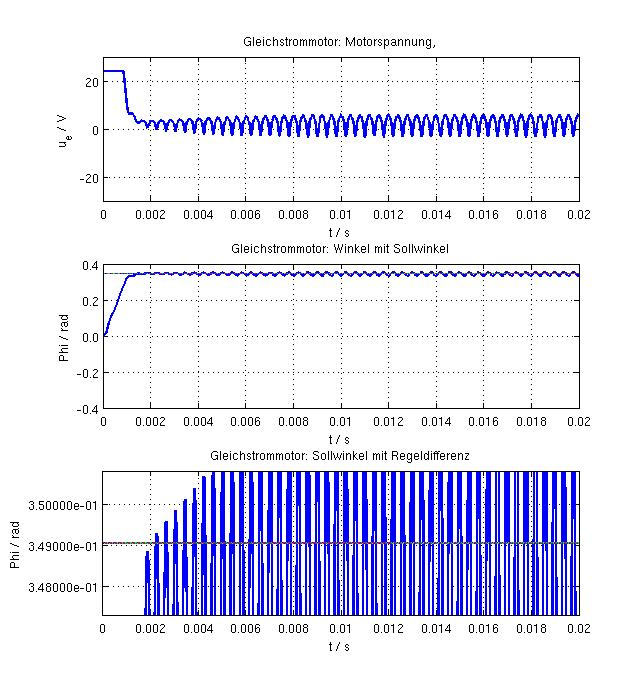
\includegraphics[width=0.6\textwidth]{Pad-Werte-P330F1_5F2_370.jpg}
	\caption{P-Adaption mit neuen Motorparametern}
	\label{padwerte}
\end{figure}

Nun werden die Motor- und Spiegelwerte solange ver�ndert, bis sich das gew�nschte Ergebniss einstellt. 
Sollte die Regelung erfolgreich sein, k�nnte mit den ver�nderten Werten evtl. ein Motor und Spiegel hergestellt werden, der den Anforderungen entspricht.

F�r die folgenden Simulationen wird das Matlab-File "msSpiegel_Pad_Neue_Werte.m" und das Simulink-File "sSpiegelPad.slx" hergenommen.

\begin{figure}[!h]
	\centering
	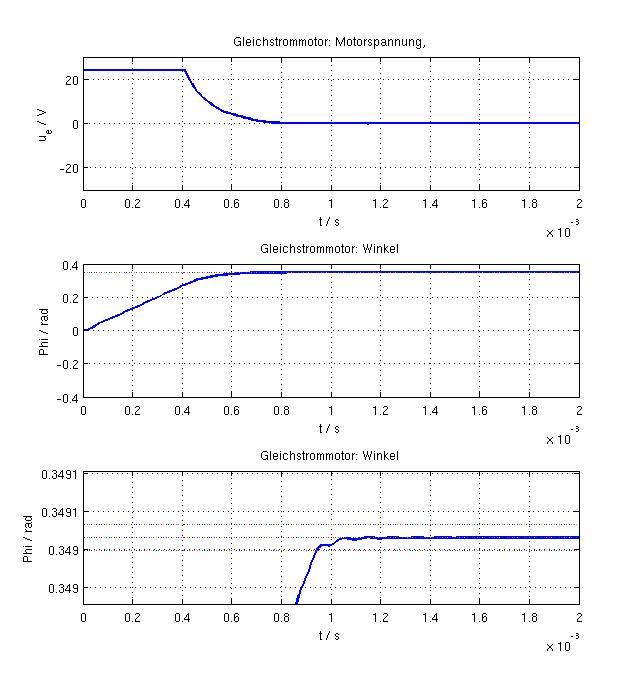
\includegraphics[width=0.6\textwidth]{Pad-Neue-Werte-P320F1_2F2_160.jpg}
	\caption{P-Adaption mit neuen Parametern}
	\label{padneuewerte}
\end{figure}

Wie in Abb. \ref{padneuewerte} zu erkennen, ist die Regelung in den geforderten Bereichen erfolgreich.
Der geforderte Winkel von 20{\textdegree} ist unter 1ms in seinen Regeldifferenzen erreicht. Dieser Regelung liegen folgende Werte zu Grunde:
Innenwiderstand der Spule: 0.1 \Omega
Induktivit�t der Spule: 3 \mu H
Motorkonstante KMPHI: 35e-3 Vs
Reibungskoeffizient: 6e-5 Nm*s
Tr�gheitsmoment des Spiegels: 93.3e-9 $kg*m^2$
Drehmoment auf den Spiegel:130.25e-6 Nm
P-Anteil: 320
$f_1$: 2
$f_2$: 160

Ein Blick auf den Strom liefert allerdings Ergenisse, die weiterer �berarbeitung bed�rfen.
In Abb. \ref{stromzuhoch} ist der Strom der aktuellen Regelung dargestellt. Es fliessen Str�me in H�he von 80 A.

\begin{figure}[!h]
	\centering
	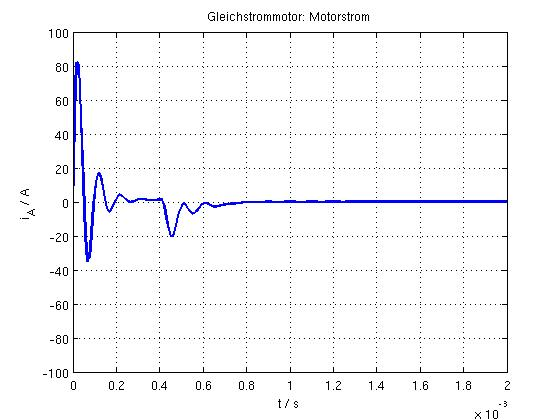
\includegraphics[width=0.6\textwidth]{Strom_zu_hoch.jpg}
	\caption{Stromh�he w�hrend der Regelung}
	\label{stromzuhoch}
\end{figure}

Dies ist allerdings sehr hoch, deshalb wird in die bestehende Regelung eine Strombegrenung von 10 A eingebaut und erneut versucht, die Regelung entsprechende anzupassen.

F�r die folgenden Simulationen wird das Matlab-File "msSpiegel_Pad_Neue_Werte_Strom.m" und das Simulink-File "sSpiegelPadStrom.slx" hergenommen.

Eine Regelung mit den aktuellen Werten zeigt das in Abb. \ref{strombegrenztpad} zu erkennende Ergebnis.

\begin{figure}[!h]
	\centering
	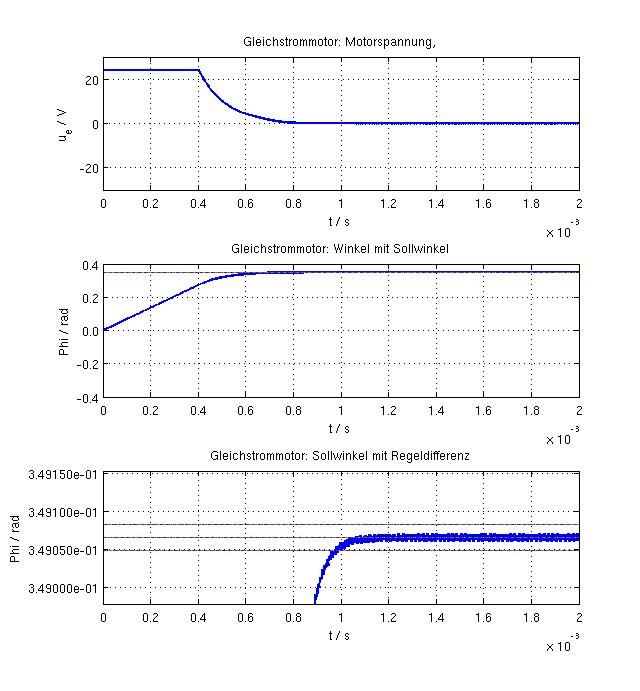
\includegraphics[width=0.6\textwidth]{Strom-Pad-Neue-Werte-P320F1_2F2_160.jpg}
	\caption{P-Adaption mit Strombegrenzung}
	\label{strombegrenztpad}
\end{figure}

Durch weiteres Anpassen der unterschiedlichen Parameter, konnten die Sollwerte fast erreicht werden. Abb. \ref{strombegrenztpadfastsoll} zeigt schon ein sehr gutes Ergebnis.
Neues Tr�gheitsmoment des Spiegels: 93.3e-11 $kg*m^2$
Neues Drehmoment auf den Spiegel: 30,25e-6 Nm
P-Anteil: 218
$f_1$: 5
$f_2$: 400

\begin{figure}[!h]
	\centering
	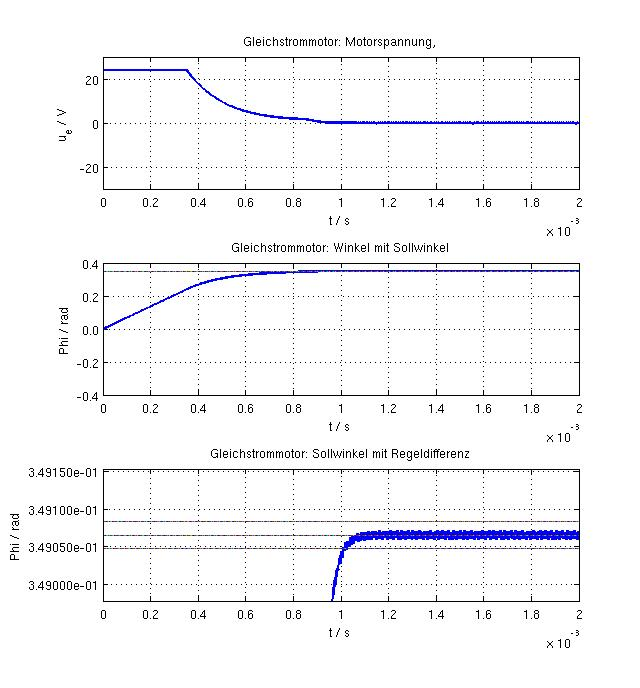
\includegraphics[width=0.6\textwidth]{Strom-Pad-Neue-Werte-P218F1_5F2_400.jpg}
	\caption{Angepasste P-Adaption mit Strombegrenzung}
	\label{strombegrenztpadfastsoll}
\end{figure}

Die Einregelzeit liegt nur noch knanpp �ber der vorgegebenen Zeit, durch weitere Anpassung der Regelparameter soll die vorgegebene Einregelzeit erreicht werden.
Abb. \ref{}
\begin{figure}[!h]
	\centering
	\includegraphics[width=0.6\textwidth]{Strom-Pad-Neue-Werte-P250F1_3F2_150.jpg}
	\caption{Angepasste P-Adaption mit Strombegrenzung}
	\label{strombegrenztpadsoll}
\end{figure}

Tr�gheitsmoment des Spiegels: 93.3e-11 $kg*m^2$
Drehmoment auf den Spiegel: 30,25e-6 Nm
P-Anteil: 250
$f_1$: 3
$f_2$: 150

In Abb. \ref{strombegrenztpadsoll} ist zu erkennen, dass durch Anpassung des Tr�gheitsmoments des Spiegels, des wirkenden Drehmoments auf den Spiegel und der verschiedenen
Regelparameter, trotz Spannungs- und Strombegrenzung, die Regelung erfolgreich ist. Der Spiegel zittert zwar etwas um die Position, dies ist aber im angegebenen 
Toleranzbereich.

\newpage
%\null
%\cleardoublepage



%************************************************************************************************
% Kap. 6 Disskussion
%************************************************************************************************

\chapter{Disskussion}
\label{chap:Disskussion}
Die Verstellung von Laserablenkspiegeln erfolgt i.d.R. durch Galvos.
In dieser Simulationsstudie sollte die Regelung eines Gleichstrommmotors zur Spiegelverstellung untersucht werden.
Die Simulationsstudie wurde mit einem vorgegebenen Gleichstrommotor Abb. \ref{fig:motoraufbau} aus Kap. \ref{chap:ganzermotor} begonnen.
F�r diesen Motor wurde ein PID-Regler in Simulink integriert, Abb. \ref{fig:grundprogramm} aus Kap. \ref{chap:motorinsimulink}, und unterschiedliche Regelparameter getestet.
Der Sensor wurde noch nicht integriert, um erst einmal eine Regelung f�r einen Gleichstrommotor zu bekommen, mit der es �berhaupt m�glich ist, einen Winkel einzustellen.

Bei der reinen P-Regelung, konnte weder die Einregelzeit, noch die Genauigkeit erreicht werden.
<<<<<<< HEAD
Wie in Abb. \ref{fig:p40} und \ref{fig:p45} aus Kap.\ref{chap:p_regelung} zu erkennen ist, beträgt die Zeit, bis der Winkel in der Nähe des Sollwertes ist, ca. \unit[7]{ms}.
Jedoch ist ein große Schwankung des Winkels zu erkennen.
Bei kleinerem P-Anteil von P = 40 ist die Abweichunng noch so groß, dass der Winkel in der unteren Grafik nicht erreicht wird.
Bei einem etwas größerem P-Anteil P = 45 ist zu erkennen, dass der Sollwinkel zwar überfahren wird, aber nicht stabil bleibt.
Die Abb. \ref{fig:p40} und \ref{fig:p45} sind hier dafür exemplarisch, dass auch bei anderen Werten keine erfolgreiche Regelung erreicht werden konnte.
=======
Wie in Abb. \ref{fig:p40} und \ref{fig:p45} aus Kap.\ref{chap:p_regelung} zu erkennen ist, betr�gt die Zeit, bis der Winkel in der N�he des Sollwertes ist, ca. $\unit[7]{ms}$.
Jedoch ist ein gro�e Schwankung des Winkels zu erkennen.
Bei kleinerem P-Anteil von P = 40 ist die Abweichunng noch so gro�, dass der Winkel in der unteren Grafik nicht erreicht wird.
Bei einem etwas gr��erem P-Anteil P = 45 ist zu erkennen, dass der Sollwinkel zwar �berfahren wird, aber nicht stabil bleibt.
>>>>>>> basti1

Die Erweiterung des reinen P-Reglers um einen I-Anteil ist in den Abb. \ref{fig:p30i17} und \ref{fig:p30i18} aus Kap.\ref{chap:pi_regelung} zu erkennen.
Durch die Erweiterung mit einem I-Anteil, hat sich die Einregelzeit auf ca. \unit[9]{ms} verl�ngert.
Auch wurde der Sollwinkel nicht erreicht.
<<<<<<< HEAD
Eine Erhöhung des P- oder I-Anteils führte dann wieder zu Schwingungen um den Sollwinkel, wie es in Abb. \ref{fig:p30i18} exemplarisch für einen leicht erhöhten I-Anteil
=======
Eine Erh�hung des P- oder I-Anteils f�hrte dann wieder zu Schwingungen um den Sollwinkel, wie es in Abb. \ref{fig:p30i18} exemplarsich f�r einen leicht erh�hten I-Anteil
>>>>>>> basti1
dargestellt ist.

Die Erweiterung des reinen P-Reglers um einen D-Anteil ist in den Abb. \ref{fig:p22d1n1} und \ref{fig:p23d1n1} aus Kap.\ref{chap:pd_regelung} zu erkennen.
Hier ergibt sich das gleiche Problem wie bei der P- und PI-Regelung.
Bis zu einer Grenze der P- und D- Anteile, ist die Regelung zu weit von dem Sollwinkel entfernt.
Wird nur ein Anteil leicht erh�ht, kommt es zu einem �berschwingen um den Sollwinkel.
Jedoch hat sich die Zeit, bis der aktuelle Winkel um den Sollwinkel schwingt, auf ca. \unit[6][ms} verk�rzt.

Es wurde nun mit einer PID-Regelung versucht, die Vorgaben zu erreichen.
In den Abb. \ref{fig:p20i15d1n1} und \ref{fig:p20i16d1n1} aus Kap.\ref{chap:pid_regelung} sind die Ergenisse der PID-Regelung dargestellt.
Es zeigt sich das von der P-, PI- und PD-Regelung bekannte Verhalten, dass bis zu entsprechenden Reglerwerten, der aktuelle Winkel zu weit vom Sollwinkel entfernt ist und
bei einer nur kleinen Erh�hung eines der Parameter, ein �berschwingen um den Sollwinkel einsetzt.
Dies ist exemplarisch f�r den I-Anteil in Abb. \ref{fig:p20i16d1n1} dargestellt.
Die Zeit bis zum ersten durchstreichen des Sollwinkels ist etwas �ber \unit[8]{ms}.

Mit dieser noch nicht zufriedenstellenden Regelung, wird der PID-Reglerblock in Simulink entfernt und eine P-Adaption in den Regelkreis eingebaut.
Abb. \ref{fig:padaptionsimulin} aus Kap. \ref{chap:padaption} zeigen diesen Aufbau.
Mit der vorgeschalteten Funktion vor den P-Verst�rker, soll eine geringere bleibende Regeldiffernz erreicht werden.

Wie aus den Abb. \ref{fig:padp41f1580} und \ref{fig:padp50f3400} aus Kap.\ref{chap:p_adaption} zu erkennen ist, wird der Sollwinkel noch nicht erreicht.
Der aktuelle Winkel gelangt bei kleineren Parameterwerten nicht in die N�he des Sollwinkels.
Bei gr��eren Parameterwerten dagegen, ergibt sich wieder ein �berschwingen um den Sollwert.
Auch mit dieser P-Adaption konnten keine Parameterwerte gefunden werden, mit der eine Regelung bei diesem Gleichstrommotor, den Vorgaben entsprechend realisiert werden konnte.

Um eine erfolgreiche Regelung zu erreichen, werden die Motorparameter angepasst, w�hrend die P-Adaption als Regelung behalten wird.
Es wird zuerst die Induktivit�t und der Innenwiderstand eines Galvos eingesetzt, um so erneut Parameter zu finden, die eine erfolgreiche Regelung erm�glichen.

Mit diesen Parametern konnte zwar ein �berschwingen um den Sollwinkel nicht verhindert werden, jedoch hat sich die Zeit, bis zum ersten durchschreiten des Sollwinkels auf
ca. $\unit[2]{ms}$ verk�rzt.
Abb. \ref{fig:padwerte} aus Kap. \ref{chap:p_adaptiongalvo} zeigt den Vorgang.

Da die Anpassung des Motors gut Ergebnisse zeigte, wird nun mit weiterer Anpassung der verschiedenen Motor- und Spiegelwerte versucht, eine erfolgreiche Regelung aufzubauen.
Durch die so erhaltenen Parameter könnte es möglich sein, entsprechende Bauteil fertigen zu lassen, um so eine Umsetzung in die Wirklichkeit zu realisieren.

Nach entsprechenden Anpassungen konnte eine erfolgreiche Regelung aufgebaut werden.
Abb. \ref{fig:padneuewerte} aus Kap. \ref{chap:p_adaptionwerte} zeigt, dass die Einregelzeit unter \unit[1]{ms} liegt und sich der aktuelle Winkel in den Regeldifferenzen 
befindet.

Ein Blick auf den Strom zeigte, dass weitere Anpassungen notwendig sind.
Es wurde eine Strombegrenzung eingebaut und neue Regelparameter probiert.
Siehe Abb. \ref{fig:stromzuhoch} und \ref{fig:strombegrenztsauber} aus Kap. \ref{chap:p_adaptionstrom}.

Nach einigen Versuchen mit ändern der verschiedenen Parameter, ist wieder eine erfolgreiche Regelung aufgebaut worden.
Der Strom ist auf \unit[10]{A} begrenzt, die Einregelzeit liegt bei \unit[1]{ms} und der aktuelle Winkel ist in den Regeldifferenzen.
Abb. \ref{fig:strombegrenztpadsoll} aus Kap. \ref{chap:p_adaptionfertig} zeigt die erfolgreiche Regelung.

Nach dem es nun möglich ist, die Vorgaben zu erfüllen, werden 3 verschiedenen Sensoren in den Regelkreis eingebracht.
Es wird mit einem idealen linearen Sensor begonnen.
An den schliesst sich ein linearer Sensor an, der über eine Faltung der Blende mit den Lichtsensoren gebildet wird.
Der dritte und letzte Sensor stellt einen nichtlinearen Sensor dar.

Abb. \ref{fig:simusensor} zeigt den Simulationsaufbau für die verschiedenen Sensoren.
Die weitere Implememtierung der verschiedenen Sensoren erfogt über Parameter in den Matlab-Files.

Als der erste lineare Sensor das aktuelle Positionssignal lieferte, musste die Regelung angepasst werden.
Mit den neuen Regelparametern konnte sogar eine noch kürzere Einregelzeit erreicht werden.
Abb. \ref{fig:linear1} aus Kap. \ref{chap:sensorregelung1} zeigt die erfolgreiche Regelung.

Ohne die Regelparameter zu ändern, wurde der zweite lineare Sensor getestet.
Die Regelung ist zwar genauso schnell, jedoch bleibt eine Regeldifferenz übrig.
In Abb. \ref{fig:linear2} aus Kap. \ref{chap:sensorregelung2} ist der Vorgang dargestellt.
Die verbleibende Regeldifferenz wird erstmal auf die diskrete Faltung zurückgeführt, bei der Rechenfehler auftreten können.

Nun wurde der dritte Sensor getestet.
Wie zu erwarten, verbleibt eine Regeldifferenz.
In Abb. \ref{fig:nonlinear} aus Kap. \ref{chap:sensorregelung3} ist der Vorgang dargestellt.
Das ist ein Bild, wie es in einem wirklichen Aufbau z.B. mit genau messbarere Laserablenkung zu entdecken wäre.
Man müsste einen Winkel einstellen, und durch die entsprechende Laserablenkung auf den wirklichen Winkel schliessen.
In der Simulation gibt es den Vorteil, dass wir uns den wirklichen Winkel anschauen.
Dieser wird dann über den nichtlinearen Sensor in ein Spannungssignal gewandelt und dem Regler zugeführt.
Insofern würde eine Veränderung der Regelparameter keine genauere Regelung bewirken.

Nur durch die Anpassung der Motorwerte, des Spiegels und mit der Verwendung eines linearen Sensors, konnte eine den Vorgaben entsprechende Regelung evaluiert werden.
Der Innenwiderstand und die Induktivität des Motors mussten verringert werden, um eine kleinere Zeitkonstante zu erhalten.
Dies liesse sich mit entsprechend weniger Windungen im Motor realisieren.
Dies würde dann gleichzeitig dazu führen, dass die durch die Drehung verursachte Spannung geringer wäre.
Durch eine bessere Ausführung der Lager, könnte der Reibungskoeffizient verringert werden.
Somit sind die in dieser Simulationsstudie getätigten Änderungen am Motor nicht nur ein ideales Wunschverhalten, sondern könnte realisiert werden.

Es wurde zudem das Drehmoment und die Trägheit des Spiegels verringert.
Beides liesse sich realisieren.
Die Trägheit des Spiegels aus auf verschiedenen Vorgaben berechnet worden.
Diese Vorgaben waren aber willkürlich.
Durch eine Verkleinerung des Masse, der Höhe oder des Durchmessers, könnte die Trägheit des Spiegels verringert werden, siehe Form. \ref{equ:J_spiegel1} aus
Kap. \ref{chap:spiegel}.
Da der Strahldurchmesser, der auf den Spiegel trifft, in dieser Studie nicht vorgegeben ist, kann ein Spiegel mit kleinerem Durchmesser und evtl. dünnerer Ausführung
verwendet werden.
Durch die Wahl eines anderen Materials könnte das Gewicht verringert werden.
Sollte der Spiegel keine geringere Trägheit aufweisen können, so wird zur Berechnung des Drehmomentes, die Beschleunigung verringert, siehe Form. \ref{equ:M_last1} aus
Kap. \ref{chap:spiegel}.

Als eine sehr strenge Bedingung ist ein linearer Sensor aufzuführen.
Es zeigte sich, dass auch bei kleinen Abweichungen von der Linearität, eine genaue Regelung nicht mehr möglich ist.
Bei Galvos, die eigentlich für solche Aufgaben verwendet werden, hat der Sensor eine Linearität von 99,9\% \cite{CaTe}.

Der hier verwendetet Integrationsalgorithmus "ode45" wurde nicht verändert.
Der Aufbau der Sensors, der ganzen Simulation und um entsprechende Regelparameter zu evaluieren, nahm schon sehr viel Zeit in Anspruch, so dass es nicht möglich war, andere
Integrationsalgorithmusse zu testen.

\newpage
%\null
%\cleardoublepage



%************************************************************************************************
% Kap. 7 Zusammenfassung
%************************************************************************************************

\chapter{Zusammenfassung}
\label{chap:Zusammenfassung}
In der vorliegenden Simulationsstudie sollte ein Gleichstrommotor auf eine bestimmte Winkelposition eingeregelt werden.
An dem Gleichstrommotor ist ein Spiegel befestigt, der einen Laserstrahl in der Fokusebene ablenkt.
Gleichstrommotoren werden i.d.R. auf eine vorgegebene Winkelgeschwindigkeit geregelt, insofern ergibt sich hier eine neue Aufgabenstellung.
Um eine in der Realität vorhandene Information über den aktuellen Winkel zu erhalten, wurde zudem ein Sensor implementiert, mit dem unterschiedliche Verhalten simuliert 
werden konnten.

Es galt die Vorgaben, den maximalen Verstellwinkel von \unit[20]{°} innerhalb einer Einstellzeit von \unit[1]{ms} auf eine Genauigkeit von \unit[1e-3]{°} einzustellen.

Nach dem ein elektrisches und mechanisches Modell von einem Gleichstrommotor erstellt war, wurde dieses Modell in Simulink umgesetzt.
Zu Beginn wurden mit einem PID-Regler verschiedene P-, PI-, PD- und PID-Reglersimulationen durchgeführt, mit denen keine der Vorgaben erfüllt werden konnte.
Die Einregelzeit lag bei ca. \unit[6]{ms}, wobei der aktuelle Winkel viel zu stark um den Sollwinkel schwankte.

Durch entfernen des PID-Reglers und implementieren einer P-Adaption sollte die verbleibende Regeldifferenz verringert werden.
Es wurden verschiedene Simulationen durchgeführt, bei denen die Vorgaben auch nicht erreicht wurden.
Es zeigte sich sogar, dass die Einregelzeit größer geworden war und die Regeldifferenz nicht wesentlich verbessert werden konnte.

Um die Vorgaben der Regelung dennoch einhalten zu können, wurden verschiedene Motorparameter verändert und neue Simulationenn durchgeführt.
Mit den veränderten Motorwerten konnte die Einregelzeit auf ca. \unit[2]{ms} verkürzt werden.
Jedoch konnte noch keine stabile Winkelposition erreich werden.

Mit weiteren Veränderungen der Motorparameter und nun auch der Spiegelparameter wurden erneut verschiedenen Simulationen durchgeführt.
Die Vorgaben konnten nun erfüllt werden.

Leider war der Strom zu hoch, weshalb eine Strombegrenzung implementiert wurde.
Nach neuen Simulationen und anpassen verschiedenster Parameter wurde erneut eine erfolgreiche Regelung realisiert.

Mit dieser erfolgreichen Regelung wurden nun verschiedene Sensoren implementiert.

Es zeigte sich, dass ein lineare übertragender Sensor von großer Wichtigkeit ist, da sonst eine bleibende Regeldifferenz verbleibt.


\setcounter{figure}{0}
\newpage
\clearpage
\setcounter{secnumdepth}{3}

\appendix
%\ihead{Anh�nge}
%\addcontentsline{toc}{section}{Anh�nge}

\chapter{Matlab-Files}

\section{msSpiegelundSensor.m}
\label{app:msSpiegelundSensorM}
\lstinputlisting{../msSpiegelundSensor.m}
\newpage

\section{sensorDaten.m}
\label{app:sensorDatenM}
\lstinputlisting{../sensorDaten.m}
\newpage

\section{frect.m}
\label{app:frectM}
\lstinputlisting{../frect.m}
\newpage

\section{gkern.m}
\label{app:gkernM}
\lstinputlisting{../gkern.m}
\newpage

\section{sensor.m}
\label{app:sensorM}
\lstinputlisting{../sensor.m}
\newpage

\section{posEingabe.m}
\label{app:posEingabeM}
\lstinputlisting{../posEingabe.m}
\newpage

\chapter{Simulink-Files}

\section{1}
\label{app:1}
%\lstinputlisting{../msSpiegelundSensor.m}

%BSP f�r Script Einbindung:
%\section{Python Script f�r die Translationsmessung}
%\label{app:PyScriptMessung}
%\texttt{\lstinputlisting[language=Python, breaklines=true]{app/DatenErfassungLangeBank.py}}
%\section{AutoIt Script f�r die Winkelmessung}

%Verzeichnisse
\setcounter{figure}{0}
\newpage
%\thispagestyle {empty}



\bibliography{lit.bib}
\bibliographystyle{unsrt}
\addcontentsline{toc}{chapter}{Literaturverzeichnis} 
\newpage
%\thispagestyle {empty}


{\small \listoffigures}
\addcontentsline{toc}{chapter}{Abbildungsverzeichnis} 
\label{Abbildungsverzeichnis}

\newpage
%\thispagestyle {empty}


{\small \listoftables}
\addcontentsline{toc}{chapter}{Tabellenverzeichnis} 
\label{Tabellenverzeichnis}


%B�rokratischer Kram
\setcounter{chapter}{0}
\newpage
\setcounter{secnumdepth}{0}
\ihead{Danksagung}
%\thispagestyle {empty}



%************************************************************************************************
% Danksagung
%************************************************************************************************

\chapter*{Danksagung}
\addcontentsline{toc}{chapter}{Danksagung}


BLABLA
\newpage
\setcounter{secnumdepth}{0}
\ihead{Eidesstattliche Erkl�rung}
%\thispagestyle {empty}

\chapter*{Eidesstattliche Erkl�rung}
\addcontentsline{toc}{chapter}{Eidesstattliche Erkl�rung} 

Wir versichern hiermit gem�� � 35 Abs.7 der Rahmenpr�fungsordnung f�r Fachhochschulen in Bayern, dass wir die vorliegenden schriftliche Arbeit mit dem Titel
\begin{center}\textbf{Simulationsstudie: Regelung eines Laserablenkspiegels}\\
\end{center} selbst�ndig
angefertigt, noch nicht anderweitig f�r Pr�fungszwecke vorgelegt und keine anderen als die angegebenen Hilfsmittel benutzt haben.\\


Alle Stellen, die dem Wortlaut oder dem Sinn nach anderen Werken
entnommen sind, haben wir in jedem einzelnen Fall unter genauer Angabe der
Quelle (einschlie�lich Internet sowie anderer elektronischer
Datensammlungen) deutlich als Entlehnung kenntlich gemacht.
Dies gilt auch f�r angef�gte Zeichnungen, bildliche Darstellungen, Skizzen und
dergleichen.\\


\begin{tabbing}

erste SpaltebbbreitbreiSpaltebbbreitbreiSpaltenb\= zweite Spalte breit zweite Spalte breit breit\kill
\\ \\ \\
............................................. 					\>.............................................\\  
Ort, Datum											\>  Unterschrift (Michael Jost)
\\ \\ \\
............................................. 					\>.............................................\\  
Ort, Datum											\>  Unterschrift (Sebastian Schleich)
\end{tabbing}


\end{document}
